% !TeX spellcheck = es_ES
%\chapter{Cap\'{\i}tulo 3}
%\chapter{Solution Proposal}
\chapter{Propuesta de solución}
En este capítulo se propone una representación basada en EP para la simulación de procesos de recobro mejorado. Con este fin, se extiende el elemento "función" definido en los EP para facilitar el desarrollo de la representación del dominio de la simulación de procesos EOR. Adicionalmente, se conceptualizan los términos derivados de las ecuaciones presentadas en el marco teórico. Posteriormente, se muestra el EP completo de la simulación y se explica por secciones los eventos que procesan la simulación.\\

Esta sección se estructura así: en la sección \ref{sec:PSNew} se presentan las subrutinas definidas por el usuario como una extensión para las funciones de los EP que permite reutilizar una representación en múltiples secciones del EP y la regla para la obtención de código a partir del nuevo elemento. En la sección \ref{sec:Concepts} se revisan los términos de cada ecuación y su traducción a los conceptos presentes en el EP junto con sus respectivas relaciones estructurales y dinámicas. En la sección \ref{sec:PS_EOR} se muestra el EP completo y se explican los eventos que procesan la simulación.

%In this section we propose one element as an extension for Preconceptual Schemas(PS) which aid the understanding of diverse elements in the oil reservoir simulation domain. In addition, we present further description of the concepts stated in the theoretical framework, with their respective representation in the elaborated PS.
%This section is structured as follows: in section  we present the added elements to PS and their usage in our represented domain. In section  we propose the representation of structural and dynamical behavior of each developed concept in the theoretical framework using PS.

%\section{Added elements to Preconceptual Schemas}\label{sec:PSNew}
%\subsection{Analyst defined subroutines}\label{sec:PS_ADS}
%Analyst defined subroutines are analyst defined functions as proposed by (ref Calle) without the return argument. They use global elements and parameters of the subroutine definition. They are defined for re-using dynamical behavior elements which appear more than once in the PS. Names of both subroutines and functions must differ from operators predefined in the PS. Graphic symbol used for subroutines is the same as used for operators and functions. In figure \# we present graphical representation of analyst defined subroutines.

\section{Extensión a las Funciones del Esquema Preconceptual}\label{sec:PSNew}
\subsection{Subrutinas definidas por el analista}\label{sec:PS_ADS}
Las subrutinas definidas por el analista son funciones tal como \cite{JCalle} propone, pero carecen de un concepto retorno ``return''. Estas utilizan elementos globales y también pueden recibir parámetros adicionales, su representación gráfica es igual a la de una función, pero en su uso no hay una asignación. En la figura \ref{fig:Subroutine} se presenta la representación gráfica y su traducción a código. %\citep{AG01}.
%Nota: Poner tabla y gráfica de uso

%\section{Conceptualization}\label{sec:Concepts}
\section{Conceptualización}\label{sec:Concepts}
En esta sección se explican los conceptos principales que resultan en la traducción de las ecuaciones algebraicas resultantes de la discretización del BOM extendido y las ecuaciones constitutivas usando el método de los volúmenes finitos. En la figura \ref{fig:Concepts} se presentan los conceptos a explicar.

\begin{figure}[h]
	\centering%
	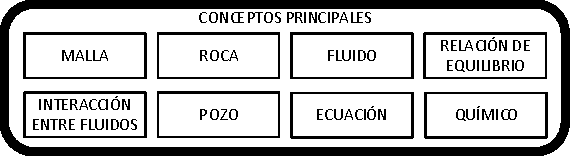
\includegraphics[width=0.9\linewidth]{Fig/Conceptos.pdf}%
	\caption[Conceptos principales en la simulación.]{Conceptos principales en la simulación. Los autores.} \label{fig:Concepts}
\end{figure}

%\subsection{Mesh}
\subsection{Malla}
Al resolver el dominio espacial continuo como un conjunto discreto de celdas (discretizar el espacio), aparecen propiedades tales como los volúmenes de las celdas y el área de las caras. Este conjunto discreto de celdas es el que se denomina como ``malla''. A su vez, la celda es vista como un conjunto discreto de caras que generan una superficie cerrada\footnote{En el caso tridimensional}. Cada celda cuenta con una numeración, esta sirve para identificar posiciones en el espacio y ubicar las vecindades correspondientes para el cálculo del flujo discretizado.\\

De la conceptualización de los elementos emergentes en la discretización, se encuentra que existe una malla. La cual, contiene todas las propiedades necesarias para generar el conjunto de celdas. Además, existe un actor ``Geomodelador'' que se encarga de definir el número de celdas en cada eje, sus espesores y topes tal como se presenta en \ref{fig:Mesh}. \\

\begin{figure}[h]
	\centering%
	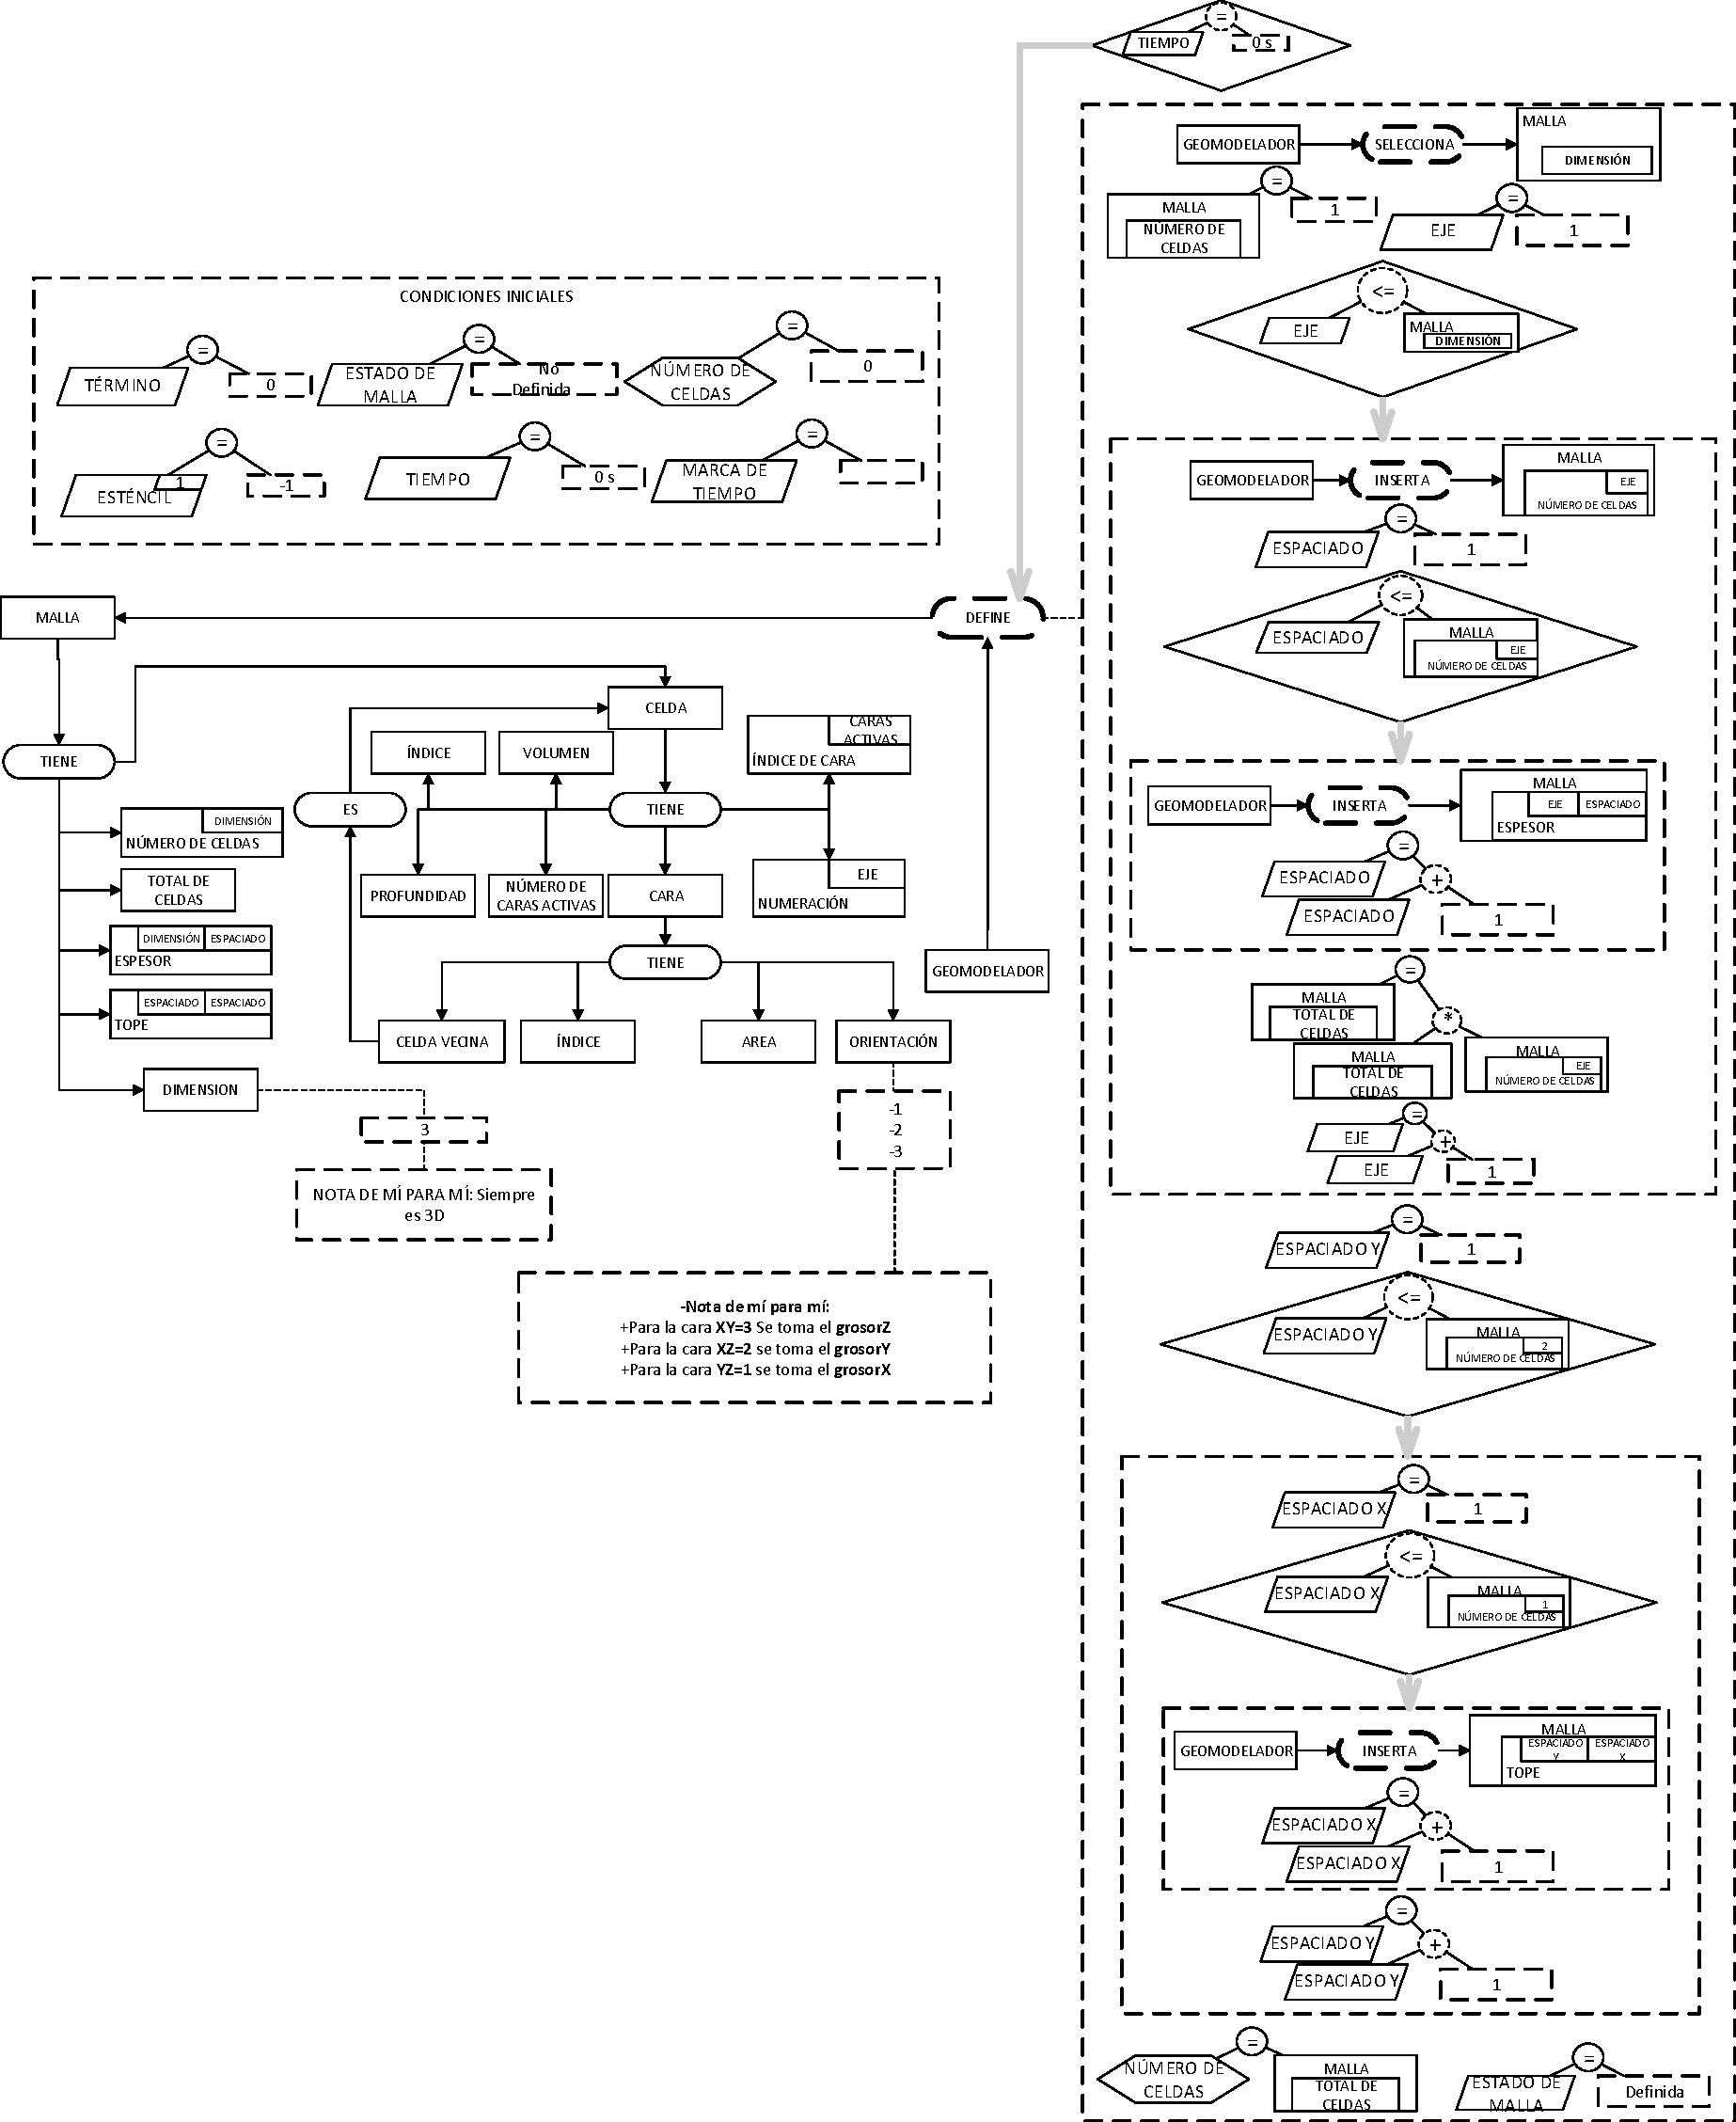
\includegraphics[width=0.9\linewidth]{Fig/Mesh.pdf}%
	\caption[Definición de la malla.]{Definición de la malla. Los autores.} \label{fig:Mesh}
\end{figure}

%Este párrafo puede servirme más para la parte del evento.
Una vez definidas tales propiedades, la malla aparece en un proceso iterativo de creación de la cantidad de celdas (Esta se presenta en el siguiente capítulo). y el respectivo cálculo de volúmenes, profundidades y numeración para cada una. Posteriormente, las caras se crean en otro proceso iterativo, estas contienen la información sobre las vecindades de cada celda, donde cada celda tiene un conjunto de caras\footnote{Es posible notar que la cara existente entre dos celdas vecinas se crea dos veces, una por cada celda.}. 

%We propose a representation of a mesh as a collection of cells which are represented likewise. collection of faces plus their respective attributes. This representation accounts for orthogonal cartesian meshes. Those are generated using the number of cells in each axis or direction, the thickness and top for each cell. Nevertheless, the thickness is only needed for the number of cells defined in every axis, because we work with regular meshes. Therefore the rest of the cells will have the same thickness.
%The top of the mesh is required for the first XY plane, and needs to be filled with the depths of each cell in that plane, the rest of the cells are calculated using the depth of the first plane.

%The representation stated for Mesh only accounts for orthogonal cartesian meshes, which can be generated with information about number of cells in each axis, their thickness and tops. A (The information above is inserted by a) Geomodeler with defines the mesh by inserting for each axis the number of cells and the thickness for cells in that direction. Once 

%\subsection{Rock}\label{sec:PS_Rock}
\subsection{Roca}\label{sec:PS_Rock}

La especificación de la relación dinámica ``Petrofísico caracteriza roca'' consiste de insertar las condiciones iniciales de porosidad y permeabilidad absoluta para la roca asociada al yacimiento, es posible notar que estos atributos de la roca están representados como arreglos por la cantidad de términos, derivados de los pasos de tiempo (estos se verán más adelante), y la cantidad de celdas definidas en la malla. \\
Adicionalmente, el petrofísico define la compresibilidad de poro y la presión a la que esta se mide para el cálculo de la porosidad a los términos posteriores. El modelo considera la existencia de una única roca a la cual todas las propiedades por cada una de las celdas son asignadas. La caracterización de la roca se presenta en \ref{fig:Rock}.\\

\begin{figure}[h]
	\centering%
	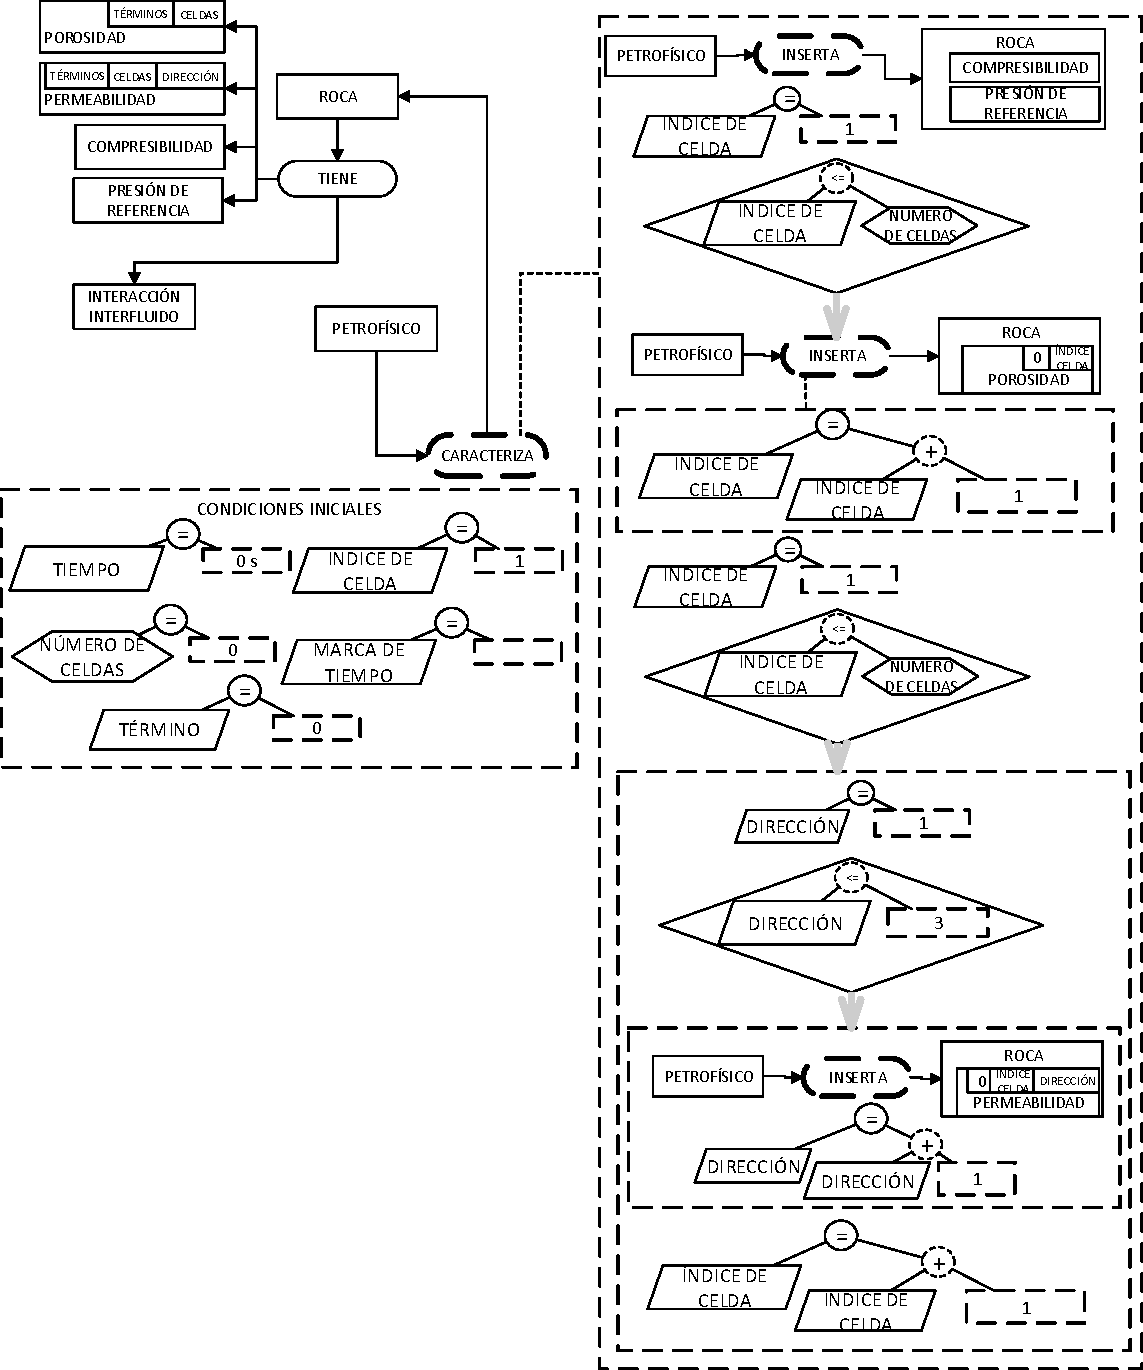
\includegraphics[width=0.90\linewidth]{Fig/Rock.pdf}%
	\caption[Caracterización de la Roca.]{Caracterización de la Roca. Los autores.} \label{fig:Rock}
\end{figure}

%\subsection{Phase}\label{sec:PS_Phase}
\subsection{Fluido}\label{sec:PS_Phase}

Los fluidos tienen propiedades que son funciones de su presión y saturación, estas a su vez son función del tiempo y del espacio. Por lo que todas las propiedades que se proponen en la conceptualización se representan como arreglos dependientes de la cantidad de términos y de la cantidad de celdas, tal como se presenta en la figura \ref{fig:FluidProps}. La representación del fluido, su relación dinámica ``Ingeniero de fluidos caracteriza Fluido'' y su respectiva especificación se presentan en la figura \ref{fig:Fluid}.\\

\begin{figure}[h]
	\centering%
	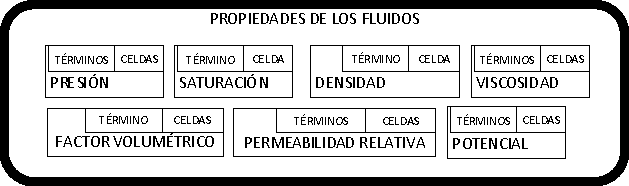
\includegraphics[width=0.9\linewidth]{Fig/PropiedadesDeFluidos.pdf}%
	\caption[Caracterización del fluido.]{Caracterización del fluido. Los autores.} \label{fig:FluidProps}
\end{figure}

\begin{figure}[h]
	\centering%
	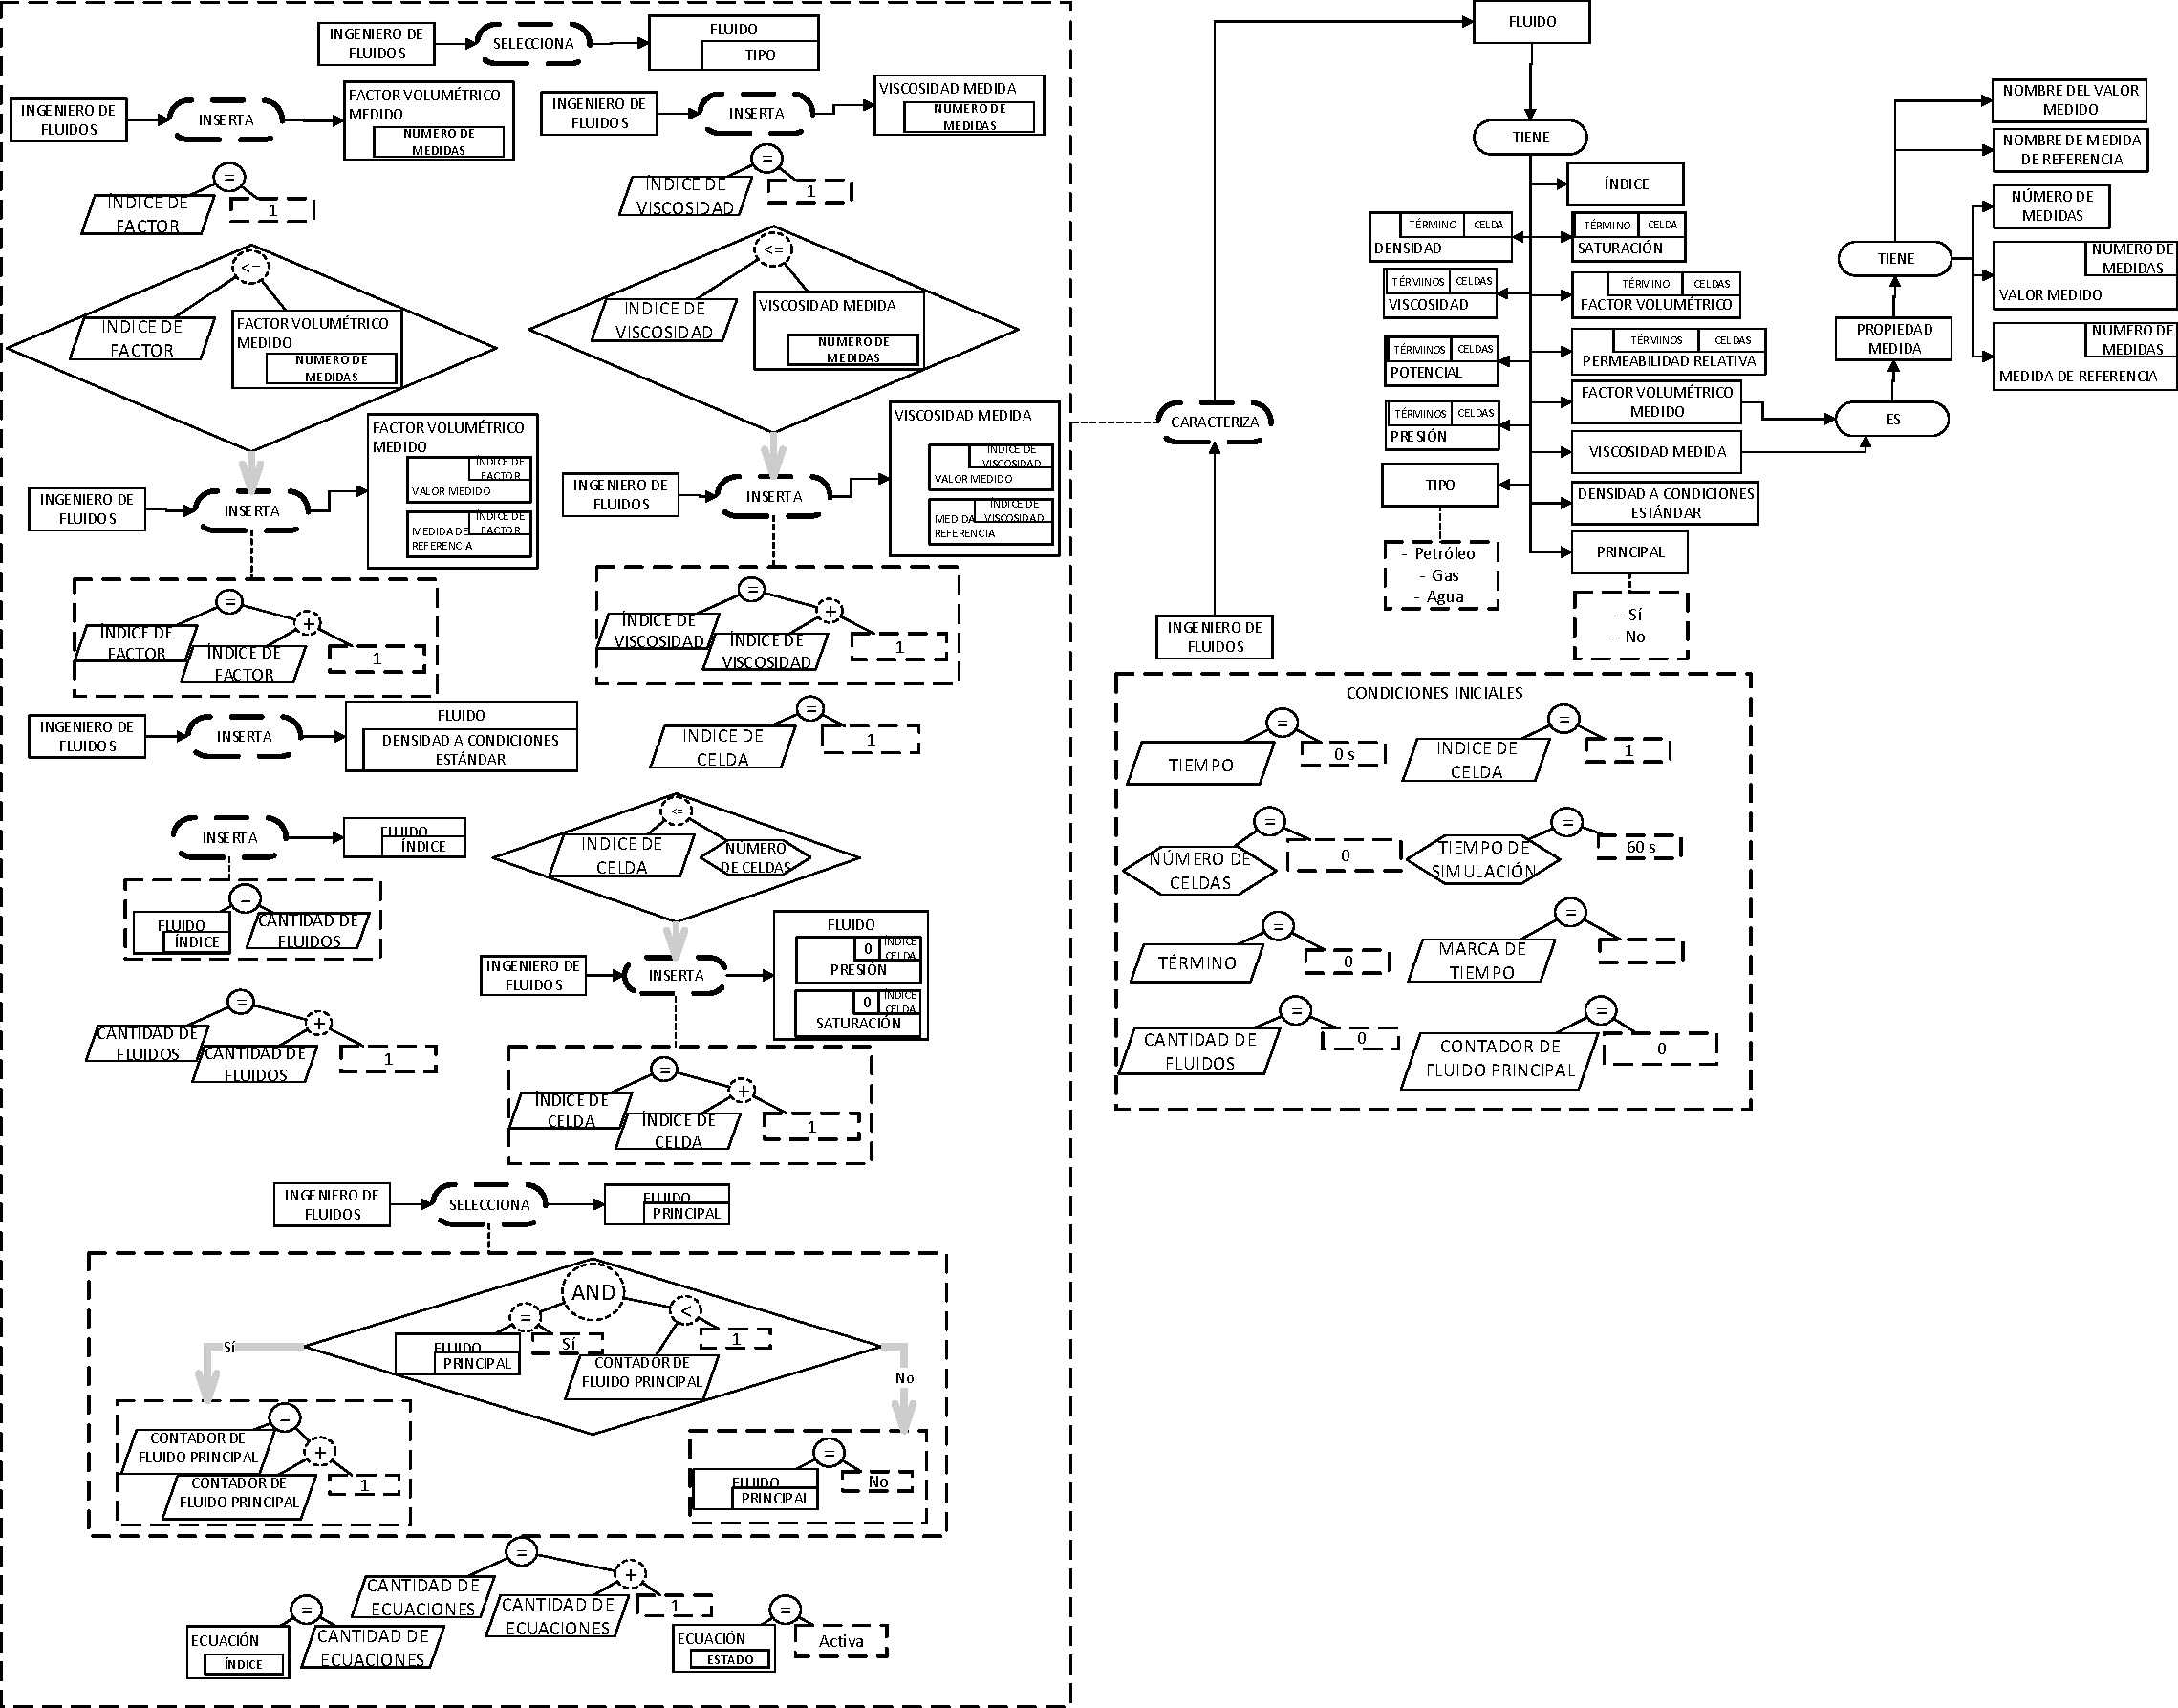
\includegraphics[width=0.9\linewidth]{Fig/Fluid.pdf}%
	\caption[Caracterización del fluido.]{Caracterización del fluido. Los autores.} \label{fig:Fluid}
\end{figure}

En pos de la generalidad, la viscosidad del fluido y su factor volumétrico se definen como funciones directas de la presión. Con este fin, aparece el concepto de ``propiedad medida'', el cuál tiene una ``medida de referencia'' y un ``valor medido'' a esa referencia. Ambos son arreglos de la ``cantidad de medidas''. En la figura \ref{fig:Fluid} también es posible ver que el fluido tiene una ``viscosidad medida y un factor volumétrico medido''. Esto nos permite calcular de manera general estas propiedades, independientemente del fluido, como una interpolación en el conjunto de medidas a la presión del fluido correspondiente. El ingeniero de fluidos inserta la viscosidad medida y el factor volumétrico medido cuando caracteriza el fluido. \\

Es importante notar también, que el fluido tiene un tipo y un atributo de tipo lógico ``Principal''. El tipo del fluido permite explicitar que este es ``petróleo'', ``gas'' o ``agua''. Sin embargo, el fluido cuyo atributo principal sea ``sí'' o ``true'', resuelve la presión en su respectiva ecuación. Los demás fluidos resuelven su saturación. 

%\subsection{Equilibrium Relation}\label{sec:PS_Equilibrium}
\subsection{Relación de Equilibrio}\label{sec:PS_Equilibrium}
En las ecuaciones del BOM se relacionan la posible existencia de masa de gas en el aceite (Rs o gas disuelto), y, en el caso del BOM extendido, la de aceite en el gas (Rv o aceite volatilizado). En el concepto ``Relación de equilibrio'', se generaliza la existencia de masa de un fluido dentro de otro fluido como un coeficiente de partición, tal como se muestra en la conceptualización (ver \ref{sec:Concepts}). Se postula, también, que existe un fluido que aporta masa y otro que la recibe, tal como se ve en \ref{fig:EqRelation}. El coeficiente de partición cumple la mismas condiciones de la viscosidad del fluido y a su vez, tiene un coeficiente de partición medido. 

\begin{figure}[h]
	\centering%
	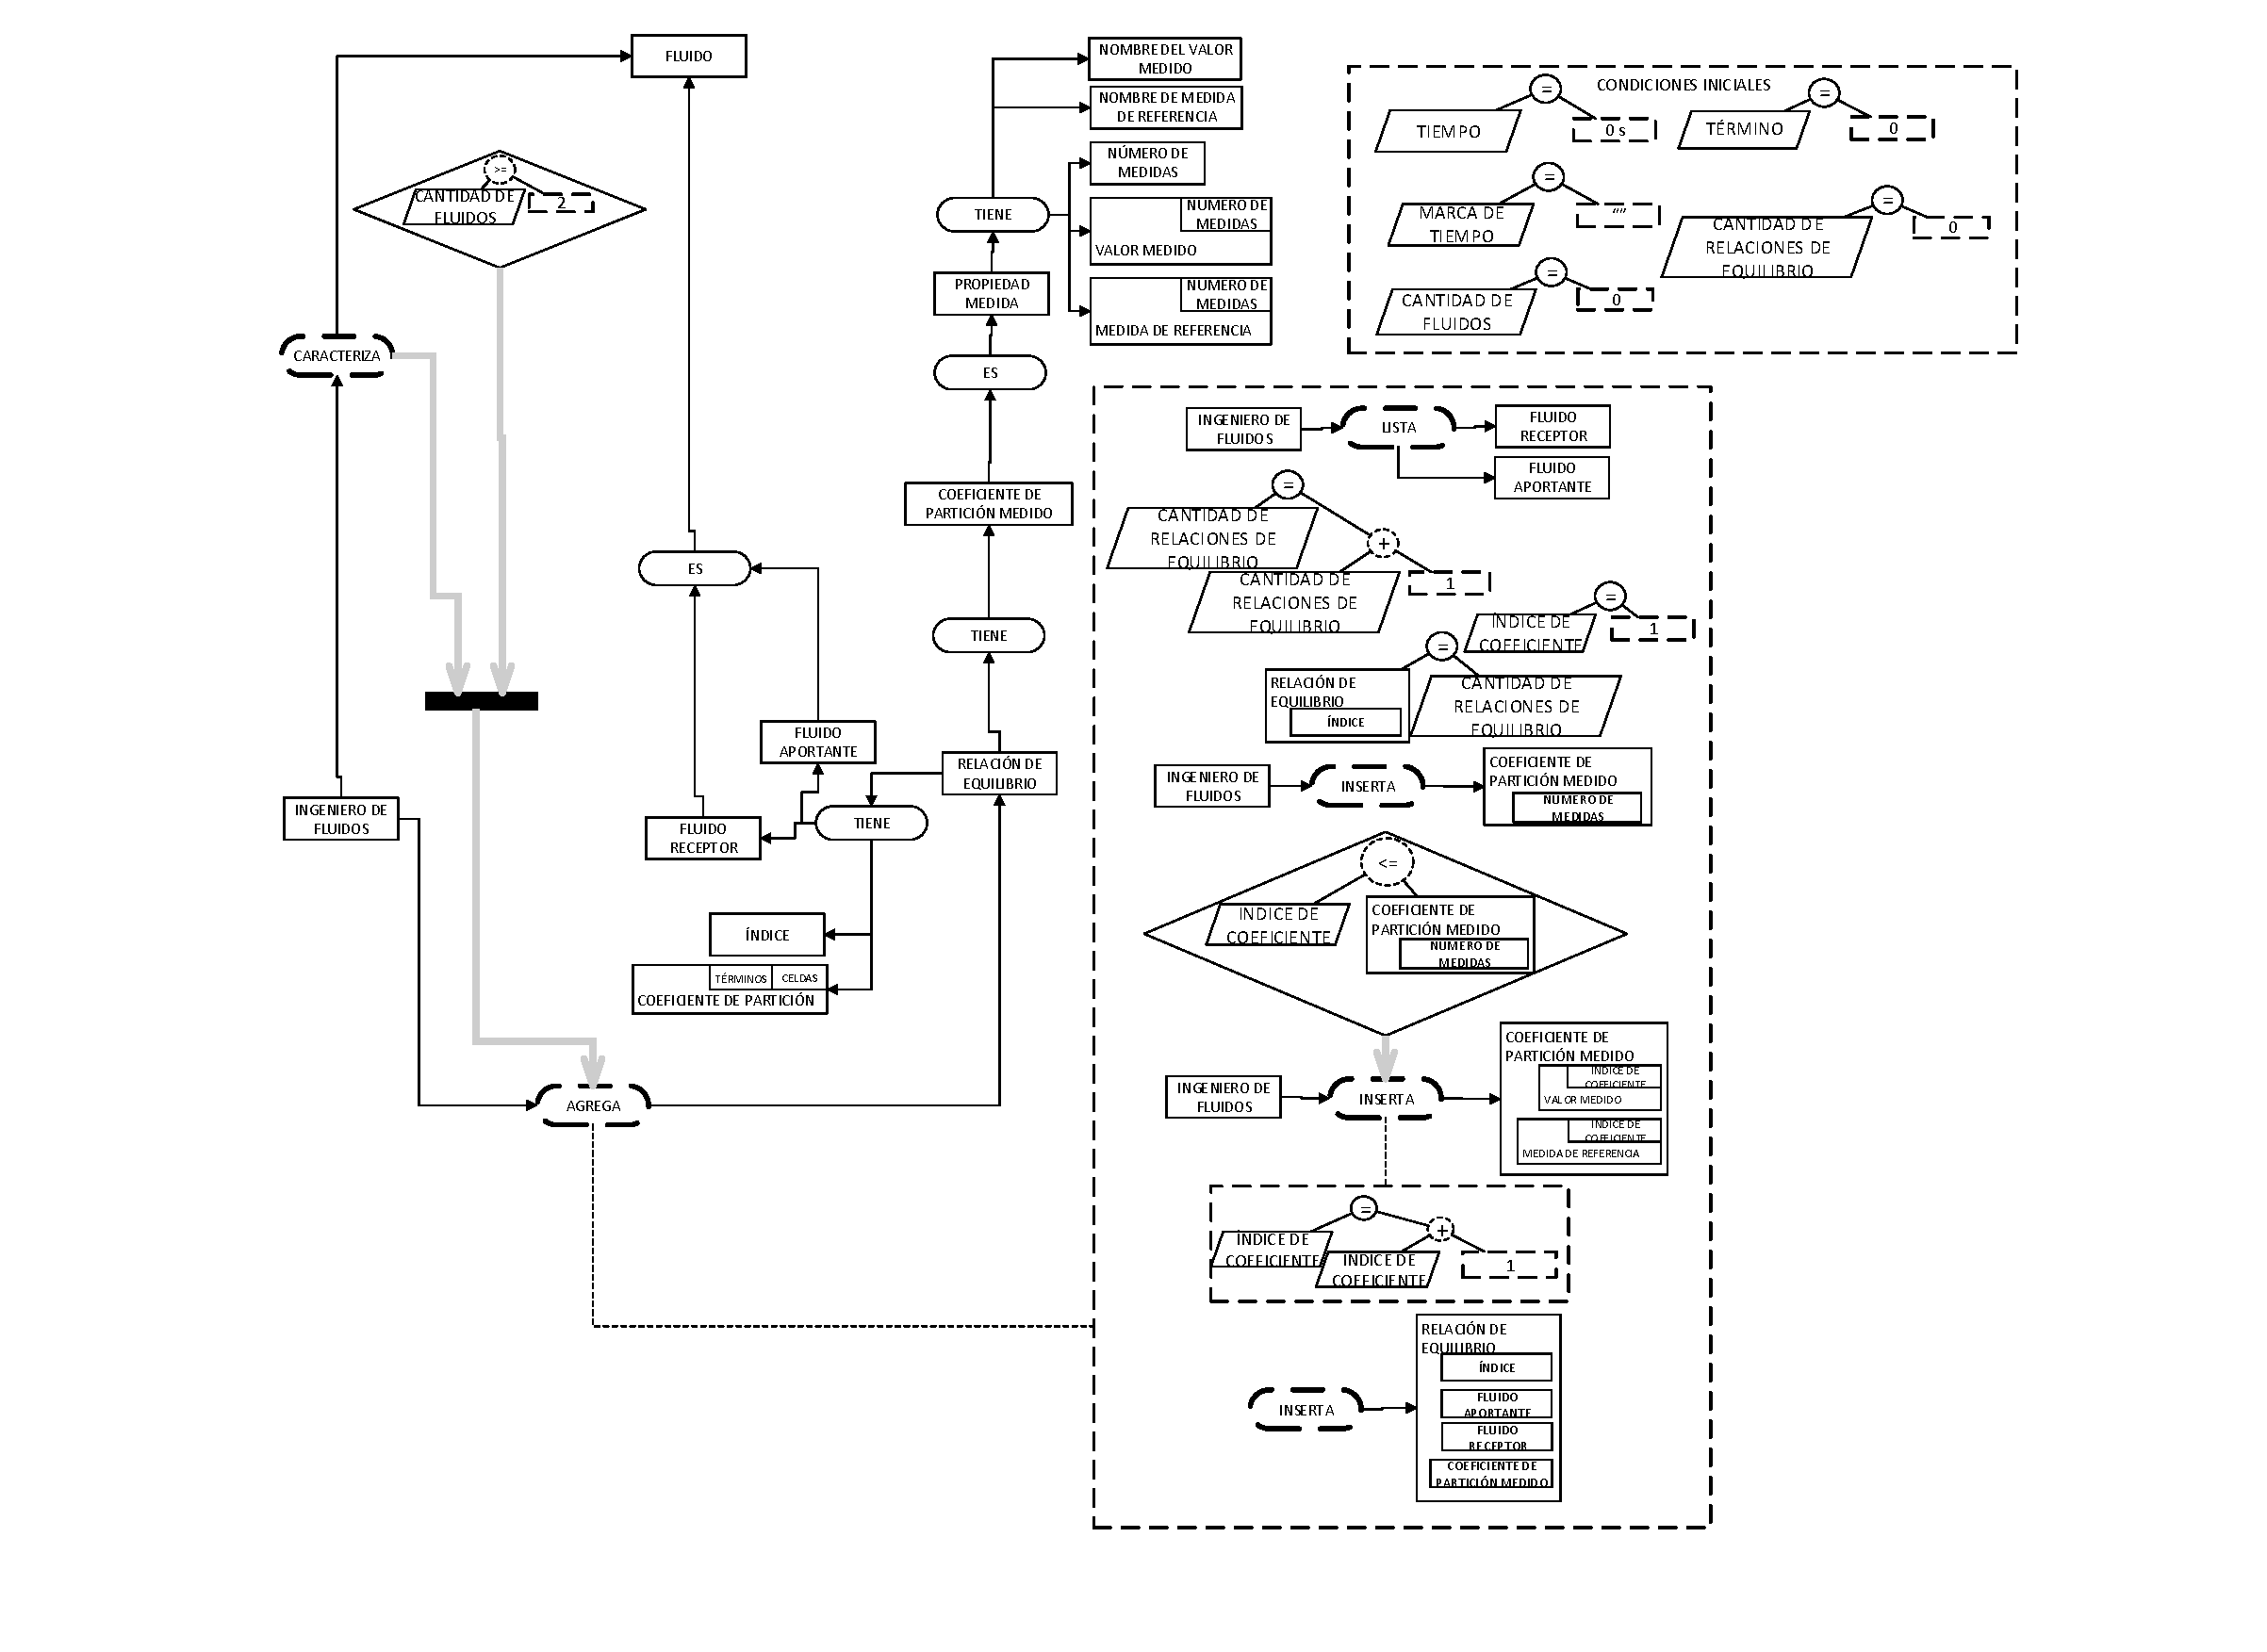
\includegraphics[width=0.9\linewidth]{Fig/Equilibrium.pdf}%
	\caption[Adición de Relaciones de equilibrio.]{Adición de Relaciones de equilibrio. Los autores.} \label{fig:EqRelation}
\end{figure}

%\subsection{Inter-phase interaction}\label{sec:PS_Interphase}
\subsection{Interacción entre fluidos}\label{sec:PS_Interphase}
%
% Qué debo mencionar acá:
% Este concepto me relaciona la presión del fluido principal con la del de referencia (Presión Capilar)
% Se espera que existan exactamente 2 para un Black Oil Model y en caso de un sistema bifásico sólo una
% Se generaliza cálculo de presiones capilares a partir de la existencia de un fluido mojante y uno no mojante.
% Se espera que uno de los dos (El fluido Mojante o el no Mojante) sea el fluido de referencia
% Todos los fluidos son claves foráneas a un fluido (No es que existan fluidos adicionales)
% Se asume que el fluido principal también es el que tiene los dos "contactos" - Hay que hablar de contactos en la conceptualización
% Las permeabilidades relativas tanto de referencia como principal y la presión capilar se interpolan a la saturación del fluido de referencia (Se verá luego).

%%%%%%%%%%%%%%%%%%%%%%%%%%%%%%%%%%%%%%%%%%%%%%%%%%%%%%%%%%%%%%%%%%%%%%%%%%%%%%%%%%%%%%%%%%%%%%%%%%%%%%%%%%%%%%%%%%%%%%%%%%%%%%%%%%%%%%%%%%%%%%%%%%%%%%%%%%%%%%%%%%%%%%%%%%%%%%%%
%NOTA: Es posible que este párrafo me sirva más para la parte de conceptualización de las Krs
%%%%%%%%%%%%%%%%%%%%%%%%%%%%%%%%%%%%%%%%%%%%%%%%%%%%%%%%%%%%%%%%%%%%%%%%%%%%%%%%%%%%%%%%%%%%%%%%%%%%%%%%%%%%%%%%%%%%%%%%%%%%%%%%%%%%%%%%%%%%%%%%%%%%%%%%%%%%%%%%%%%%%%%%%%%%%%%%
Las interacciones entre fluidos se proponen como una generalización de los contactos entre fluidos. En el caso del modelo BOM, se deben especificar dos: los contactos gas-aceite y aceite-agua. En este concepto se relacionan directamente las dependencias de la permeabilidad relativa del fluido principal con su respectivo fluido de referencia en el contacto. Además, para el fluidos cuya incógnita es la saturación, se relaciona la presión del fluido principal con su respectiva presión capilar, con el fin de calcular la presión faltante. Para esto, es necesario saber de antemano cuál fluido es el mojante y cuál es el no mojante. Adicionalmente, todas las propiedades dependientes se calculan a la saturación del fluido de referencia. En la figura \ref{fig:Contact} se presenta la representación propuesta para las interacciones entre fluidos.

\begin{figure}[h]
	\centering%
	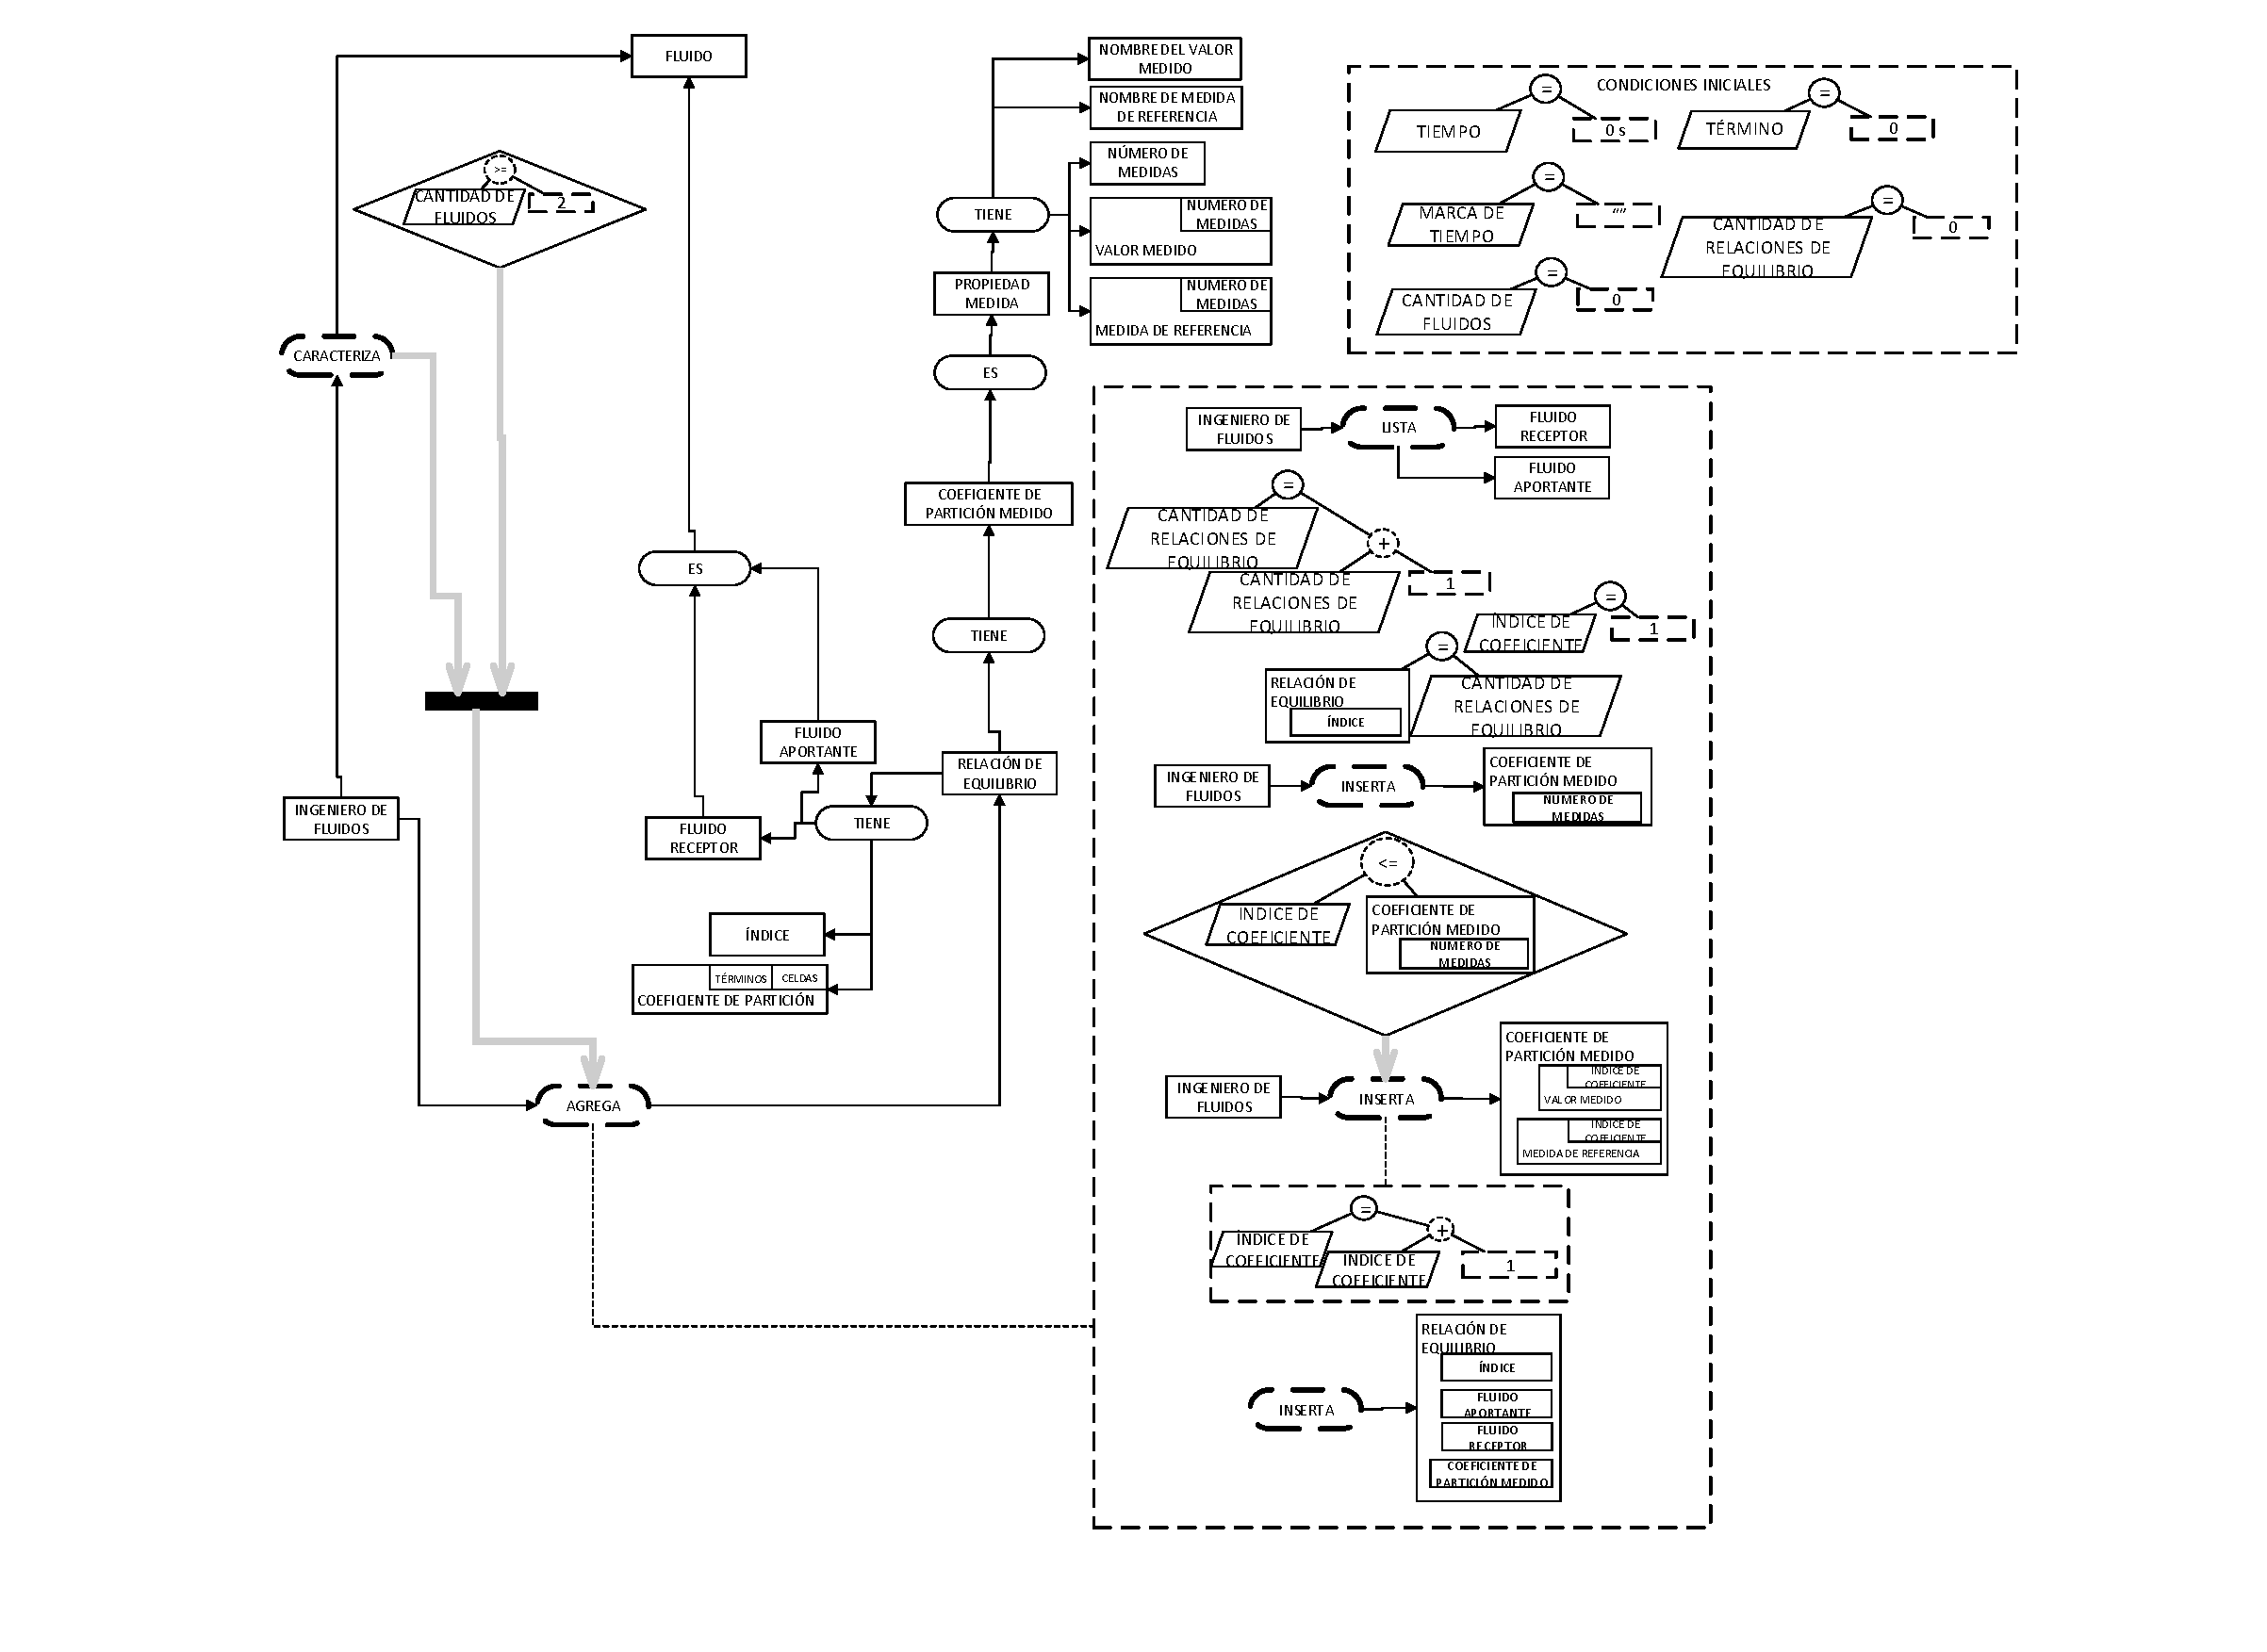
\includegraphics[width=0.9\linewidth]{Fig/Equilibrium.pdf}%
	\caption[Adición de Interacción entre fluidos.]{Adición de Interacción entre fluidos. Los autores.} \label{fig:Contact}
\end{figure}
%este concepto me relaciona un fluido de referencia, que se espera diferente del fluido con la propiedad de ser ``Principal'' y es respecto al cual se interpolarán las permeabilidades relativas, tanto propias como del fluido principal.
%\subsection{Component}\label{sec:PS_Component} % This could be changed to Chemical
%\subsection{Well}\label{sec:PS_Well}
\subsection{Pozo}\label{sec:PS_Well}
Se proponen los pozos, de manera análoga a la malla, como un conjunto de perforados que a su vez tienen atributos adicionales como lo son la presión de fondo y el caudal. Estos pozos, tienen una caracterización distinta según el tipo, sea productor o inyector. Además, es posible notar que el pozo es un concepto abstracto, de cuál se instancia uno de los dos tipos. Más aún, los perforados dependerán del tipo de pozo, siendo estos también abstractos, con sus respectivos tipos ``perforado inyector'' o ``perforado productor''. En la figura \ref{fig:Well} se presenta la representación de los pozos.\\

\begin{figure}[h]
	\centering%
	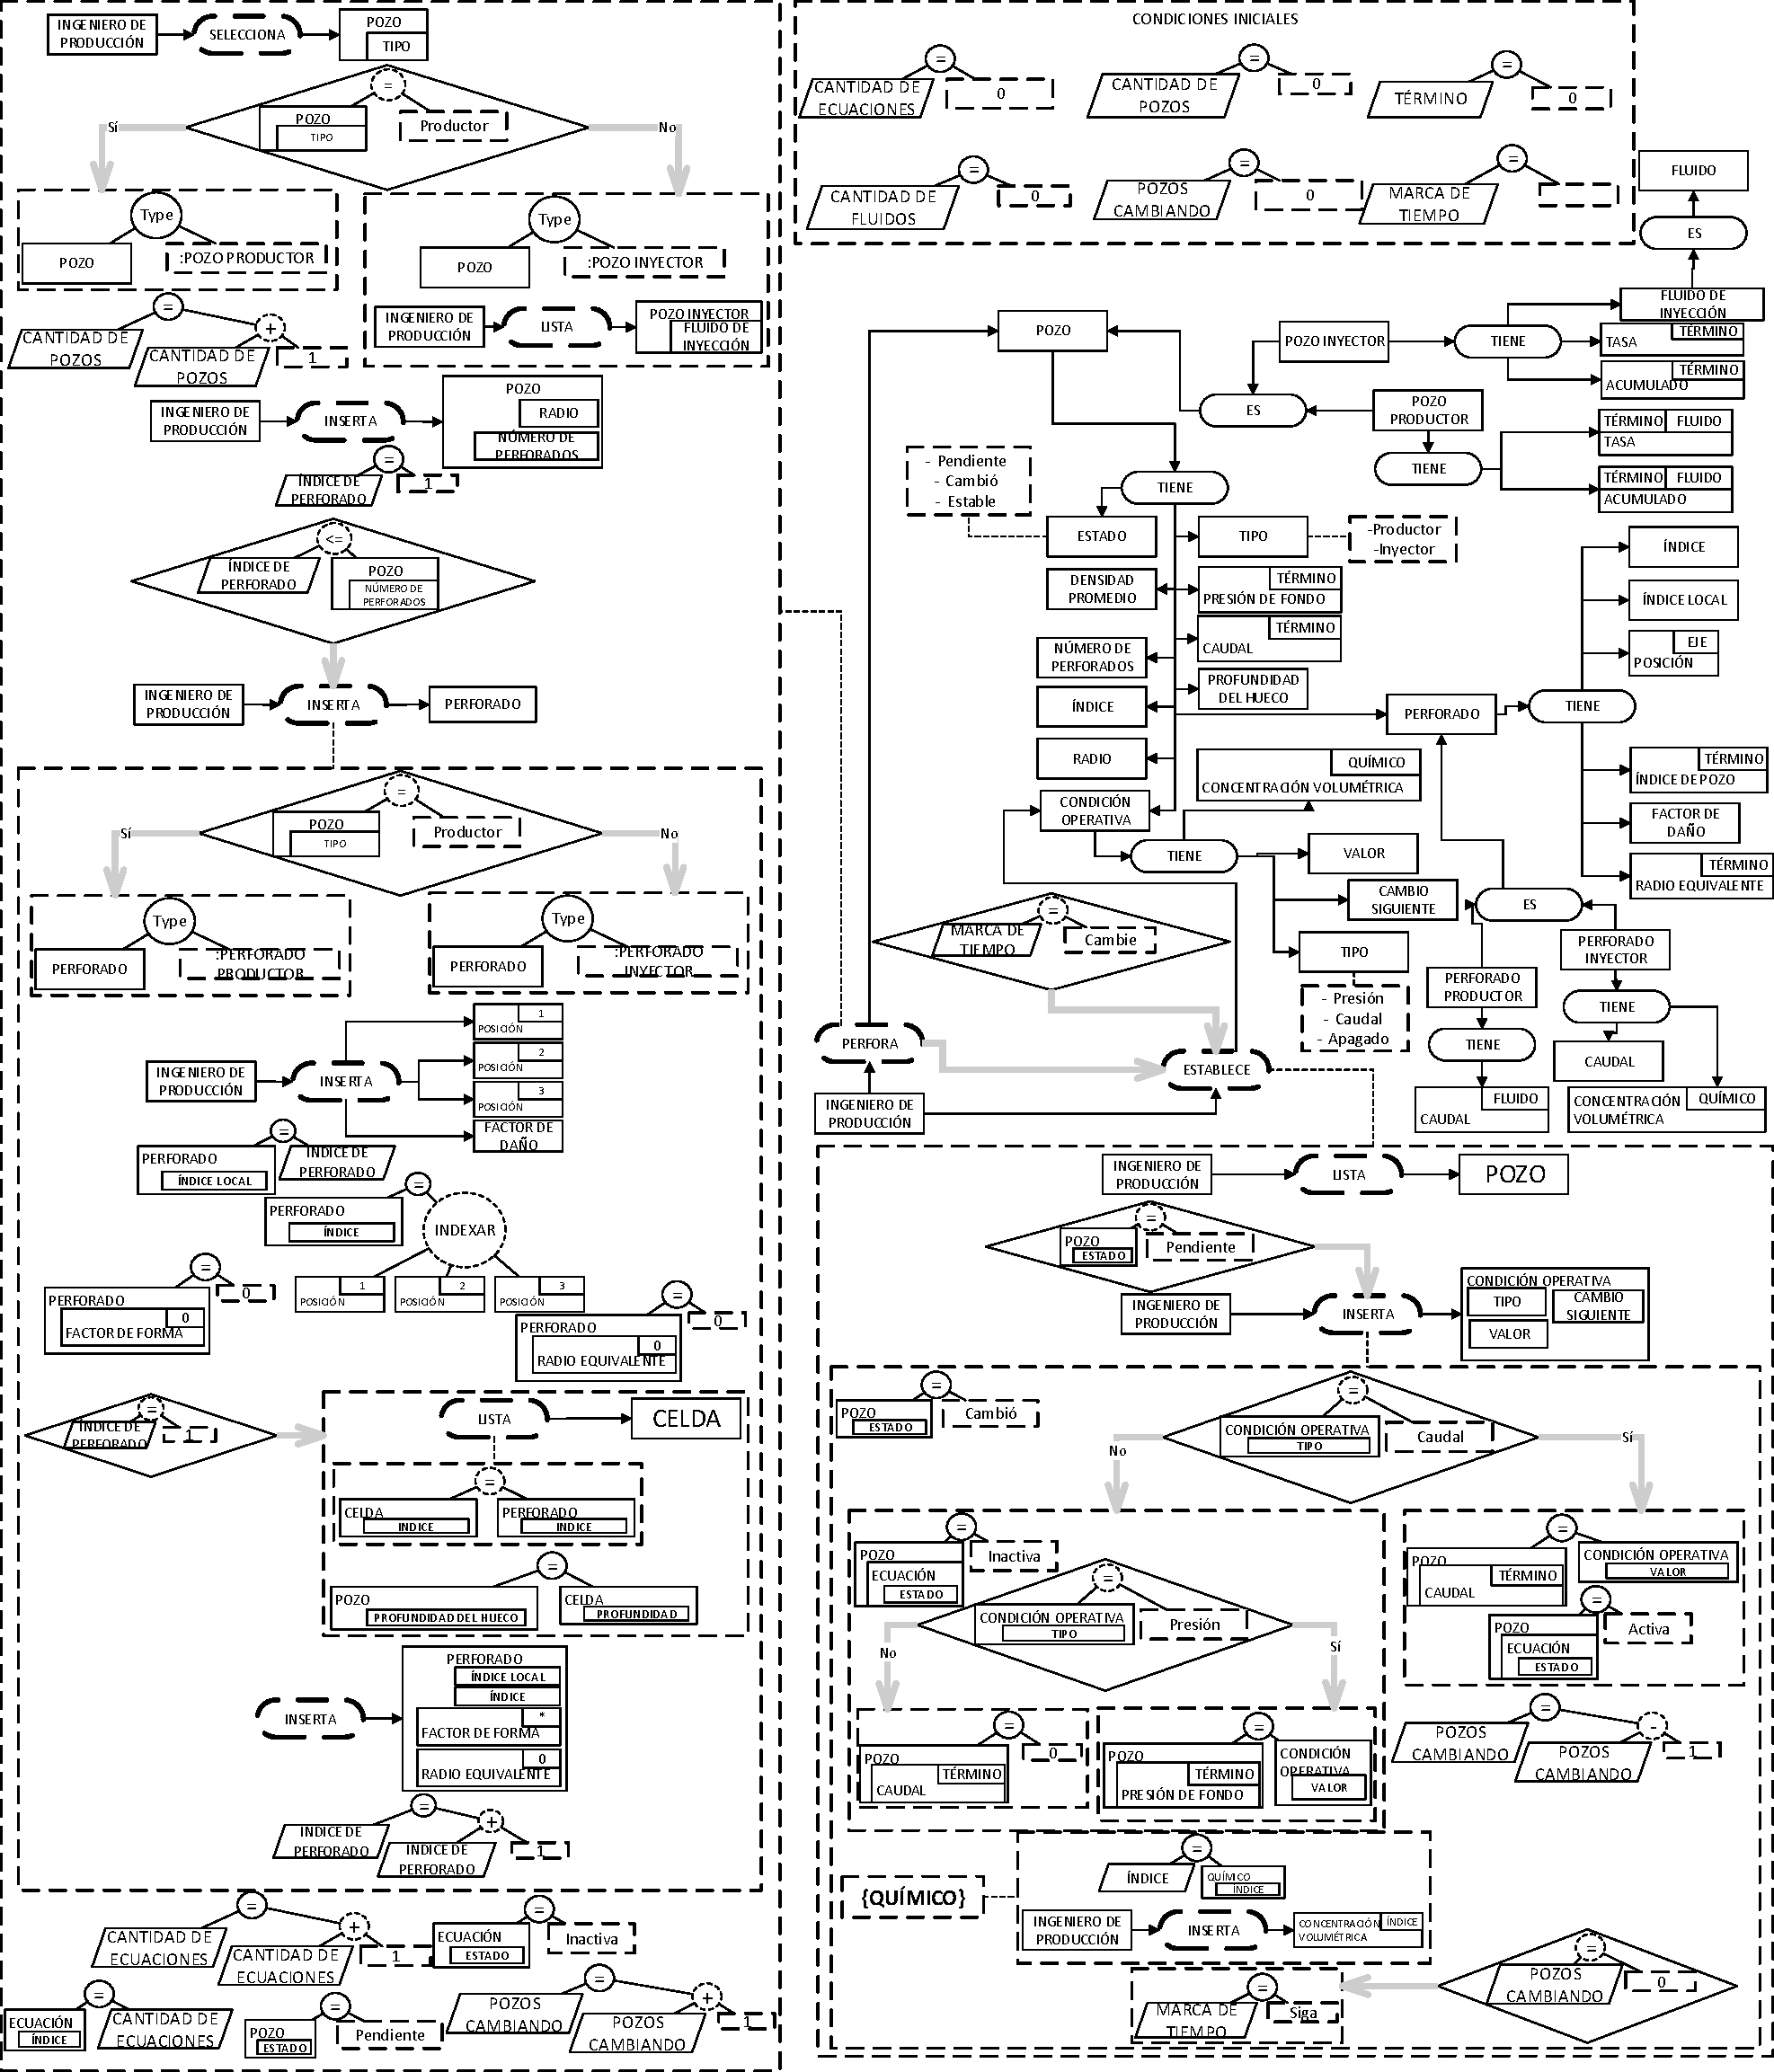
\includegraphics[width=0.9\linewidth]{Fig/Pozo.pdf}%
	\caption[Perforación de Pozos.]{Perforación de Pozos. Los autores.} \label{fig:Well}
\end{figure}

La principal diferencia entre los pozos productores e inyectores radica en que el pozo inyector tiene un fluido de inyección. Además, la tasa y el acumulado del pozo inyector sólo dependen de este fluido, mientras que para el pozo productor dependerá de la cantidad de fluidos caracterizados. Estos pozos están sujetos a la restricción de no cambiar su tipo, además para un pozo productor, su conjunto de perforados corresponderá también a perforados productores. Así mismo para los pozos inyectores.\\

Los pozos funcionan bajo una condición operativa, que permite regular la presión o el caudal al que estos inyectan o producen fluido. Estas condiciones definen si un pozo genera una ecuación (Peaceman), o si su caudal se puede resolver directamente usando la presión de fondo. Por otro lado, las condiciones operativas pueden variar en el tiempo, por lo que se requiere calcular o resolver el atributo que no está sujeto a la condición operativa cada que se establezca un cambio en esta. Adicionalmente, se reconfigura la simulación cada que se establezca un cambio en la condición operativa.

\subsection{Ecuación}\label{sec:PS_Equation}
La ecuación es un concepto agrupador, tanto el fluido como el pozo son ecuaciones (Posteriormente los químicos). Sirve para iterar sobre todos los conceptos que generan un residual en el método de Newton. Tienen un índice y estado. Este último permite que todos los pozos generen ecuación pero no necesariamente se resuelva en el jacobiano. Sólo se resuelven las ecuaciones cuyo estado sea ``activo''. (Se verá más adelante).
%Poner ecuación acá con Volumen de celda ya como concepto

%\subsection{Rock}

%\section{PS Representation of Enhanced Oil Recovery Simulation}\label{sec:PS_EOR}
\section{Representación en EP de la simulación de procesos EOR}\label{sec:PS_EOR}
En esta sección se propone una representación basada en un EP para procesos EOR. En el esquema \ref{fig:PSComplete} se evidencia la solución del BOM discretizado usando volúmenes finitos en una malla cartesiana ortogonal. El paso a paso en la ejecución de los eventos se muestra en \ref{fig:EventsInteraction}.  En el evento ``Presión del fluido varía'' se desarrollan las iteraciones del método de Newton-Raphson e internamente las iteraciones sobre las celdas requeridas para solucionar el sistema algebraico resultante de la discretización. En las secciones siguientes se explica el EP elaborado en las respectivas porciones correspondientes a eventos, subrutinas y funciones que procesan la simulación de procesos EOR. \\

Para el correcto desarrollo de la simulación, se establecen las siguientes precondiciones: existe una única malla y una única roca. En el caso de una simulación de dos fluidos debe existir una única interacción entre fluidos. En el caso de tres fluidos deben existir exactamente dos interacciones entre fluidos.


%In this section we propose a PS representation for enhanced oil recovery simulation, we couple a black oil model discretized using finite volumes method with the theoretical framework developed the previous chapter. We mapped each term in the resultant equations to their respective concepts and how they are linked together. The complete representation is shown in \ref{fig:PSComplete}.\\
\begin{figure}[h]
\centering%
\includegraphics[width=0.9\linewidth]{Fig/PozosConEcuacion.pdf}%
%\caption{Complete PS Representation for EOR Processes} \label{fig:PSComplete}
\caption[Representación en EP de la simulación de procesos EOR.]{Representación en EP de la simulación de procesos EOR. Los autores.} \label{fig:PSComplete}
\end{figure}

\begin{figure}[h]
	\centering%
	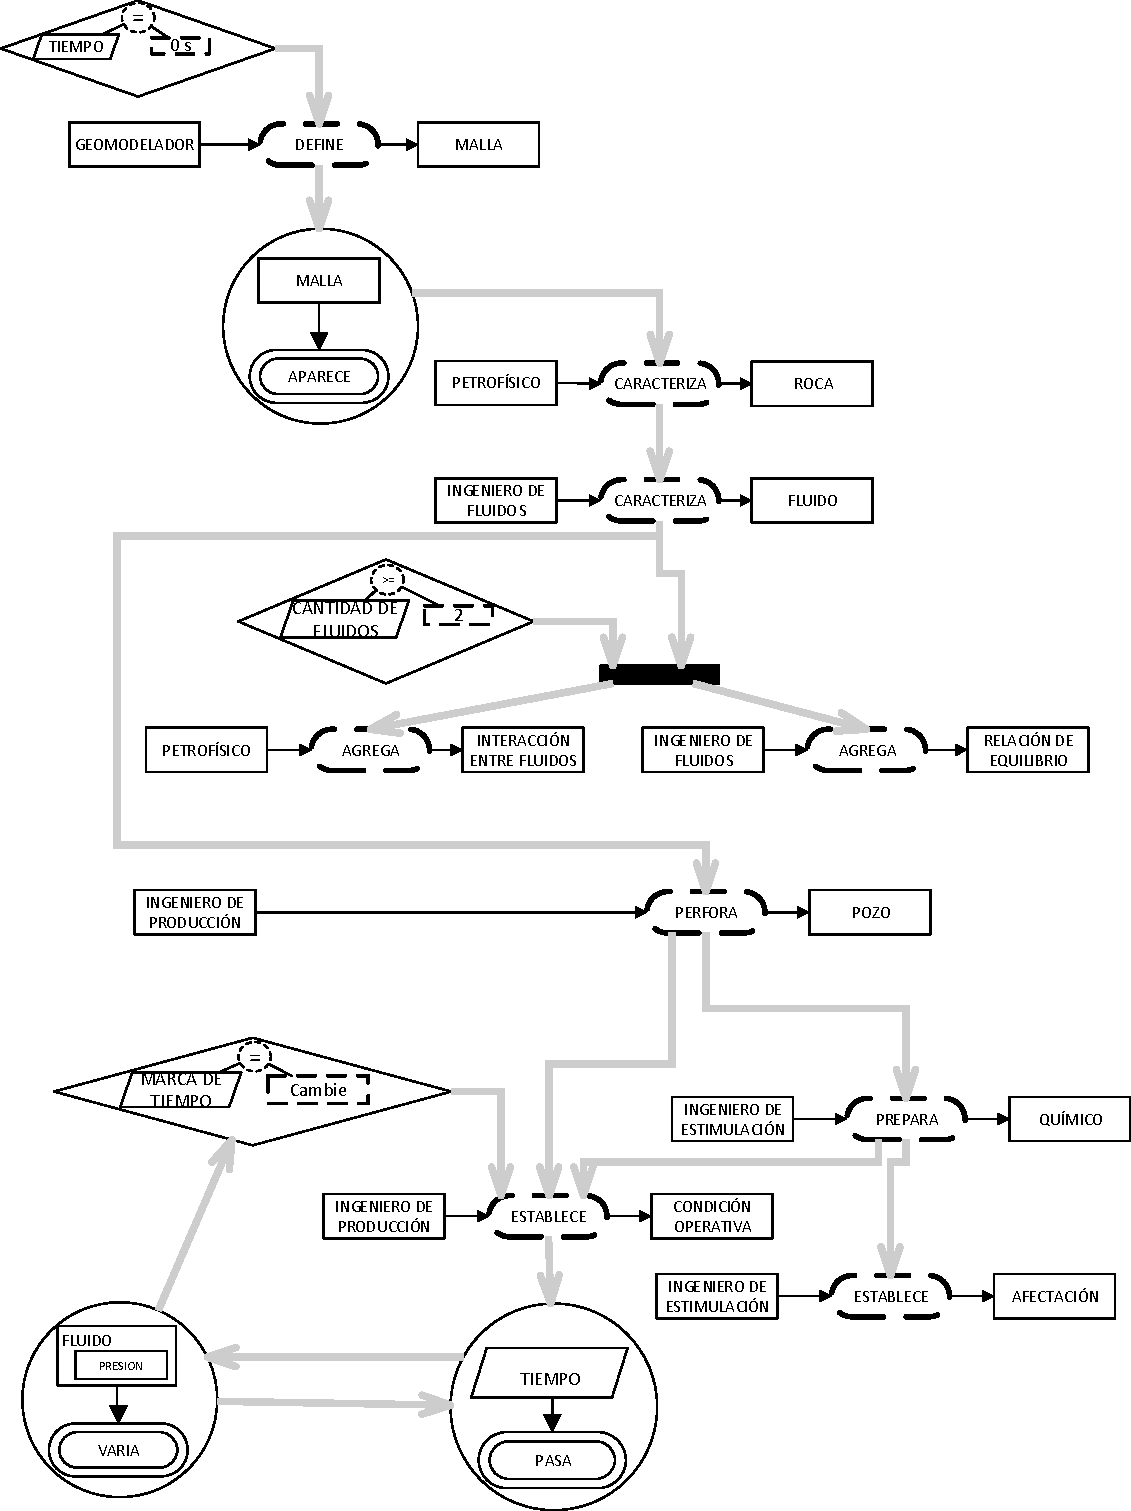
\includegraphics[width=0.9\linewidth]{Fig/FlujoDeEventos.pdf}%
	%\caption{Complete PS Representation for EOR Processes} \label{fig:PSComplete}
	\caption[Diagrama basado en el grafo de interacción de eventos.]{Diagrama basado en el grafo de interacción de eventos. Los autores basados en \cite{zapata2013Eventos}.} \label{fig:EventsInteraction}
\end{figure}
%The rest of this section is as follows: In section \ref{sec:PS_Mesh} we present the Mesh concept as a collection of cells with additional elements needed for calculating the attributes of each cell. Furthermore, we develop the dynamical relationship ``Geomodeler defines Mesh'' as an interaction of the role ``Geomodeler'' with atomic\footnote{atomic as is stated by \cite{AG01} (Aca debe ir Zapata)} dynamical relationships. In section \ref{sec:PS_Rock} we present the Rock concept with its attributes and initial characterization. In section \ref{sec:PS_Phase} ... In section \ref{sec:PS_Interphase} ... In section \ref{sec:PS_Equilibrium} we define the partition coefficients as relations between two phases, one contributing mass and another receiving mass in the mass balance equation. In section \ref{sec:PS_Well}
\subsection{Malla aparece}\label{sec:PS_MeshAppears}
El evento ``Malla aparece'' Se dispara cuando el estado de la malla es ``Definida'', que sucede justo después de que el geomodelador defina la malla. En este evento, se desarrollan dos ciclos principales. El primer ciclo es anidado por cada eje coordenado, y en total se recorre el número de celdas a definir. En este ciclo, se calculan los volúmenes y profundidades de cada celda, además se asigna un índice único de celda y la numeración en cada eje (x,y,z). La especificación del evento ``Malla Aparece'' se presenta en la figura \ref{fig:Concepts}.\\

\begin{figure}[h]
	\centering%
	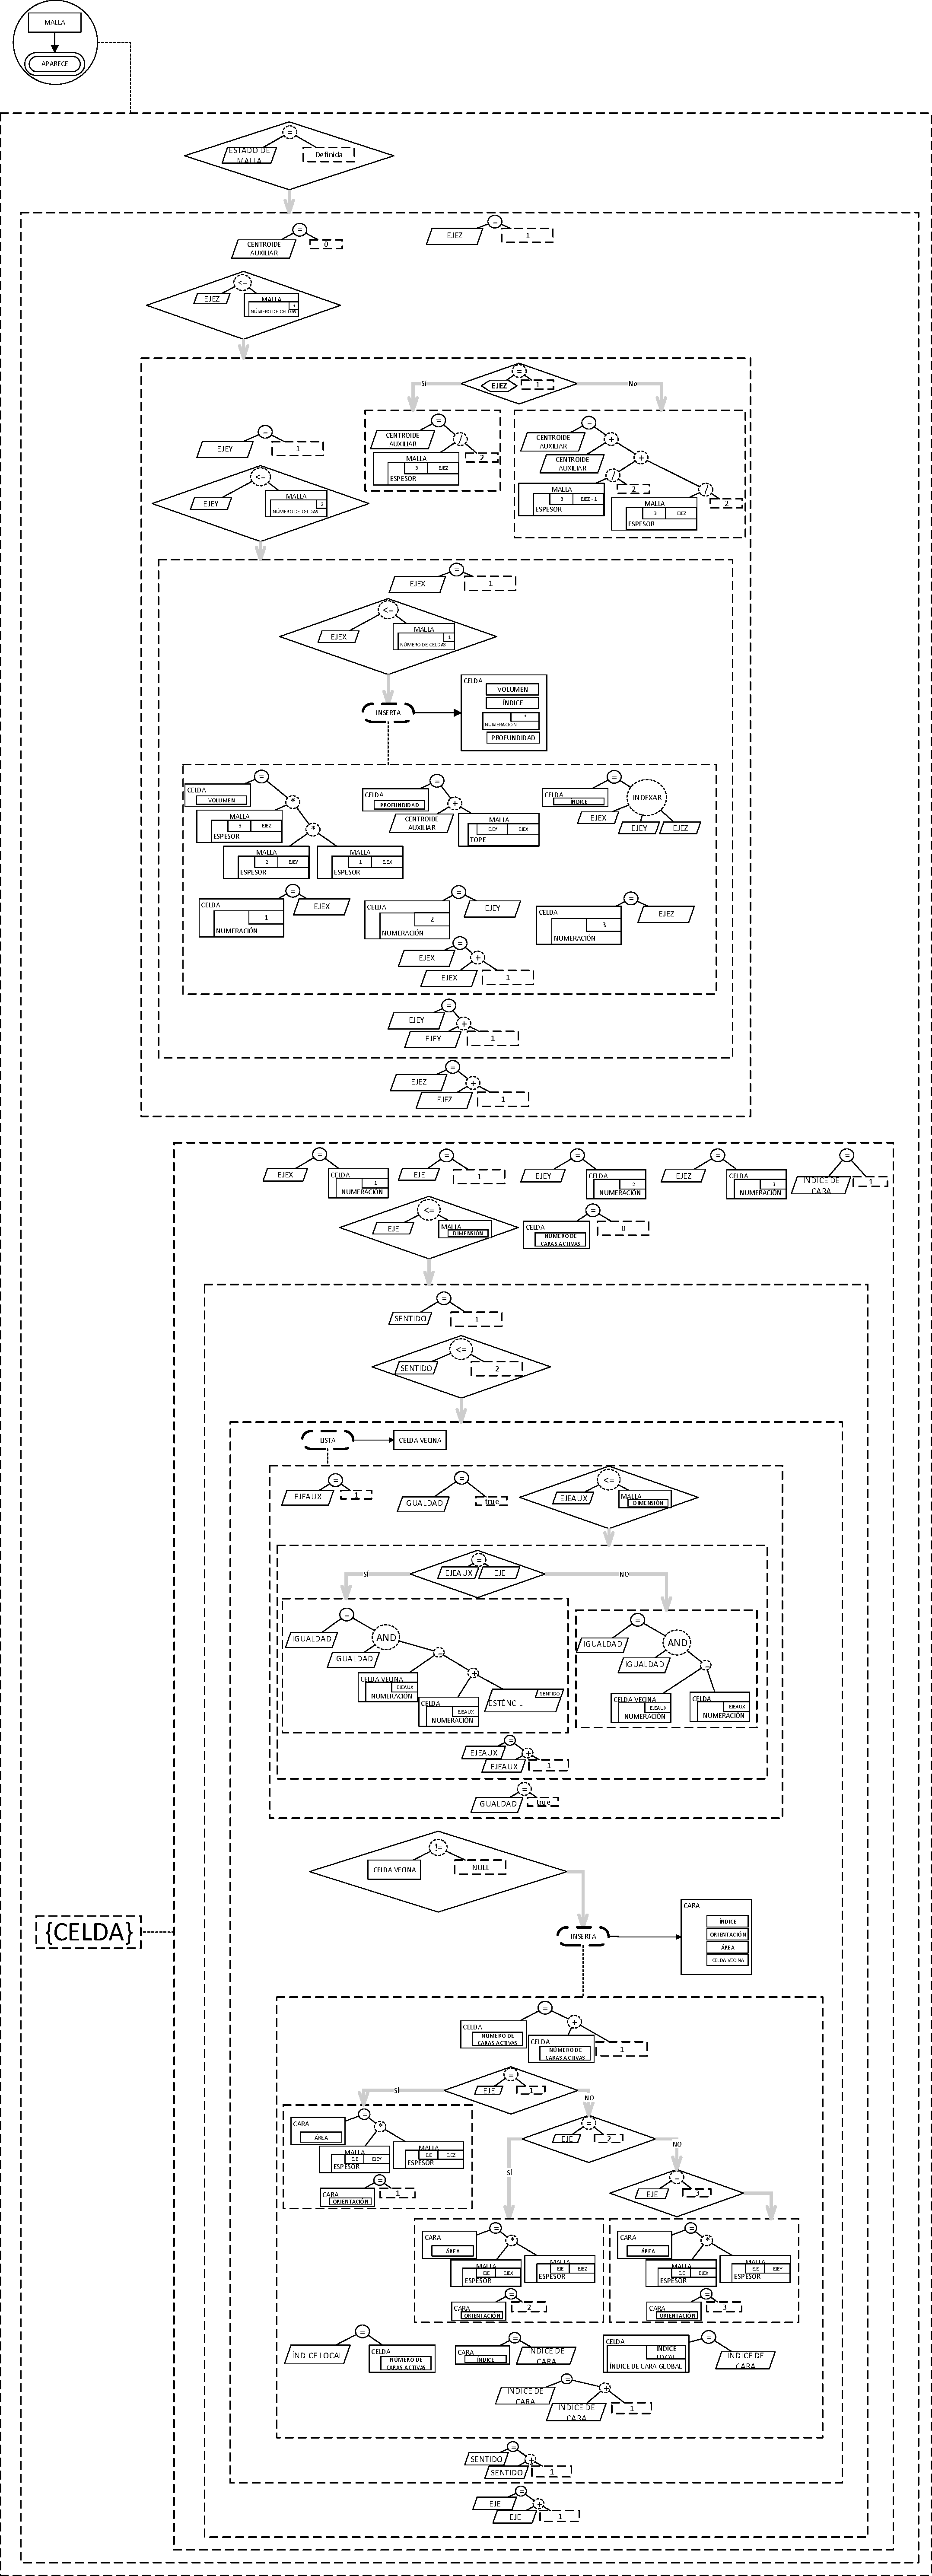
\includegraphics[height=\textheight]{Fig/MallaAparece.pdf}%
	%\caption{Complete PS Representation for EOR Processes} \label{fig:PSComplete}
	\caption[Representación de la aparición de la Malla.]{Representación de la aparición de la Malla. Los autores.} \label{fig:MeshAppears}
\end{figure}

En el segundo ciclo principal, se itera sobre las celdas definidas previamente y se calcula la conectividad, es decir la definición de caras. Para esto, se consulta la existencia de celdas adyacentes a la celda actual en todas las direcciones. Si existe una celda en alguna dirección, se crea y calcula su área y orientación. Adicionalmente, a la cara se le asigna un índice y también se le asigna la celda vecina. Es importante notar que cada celda almacena su conjunto de caras, por lo que las caras se duplican.

\subsection{Tiempo pasa}\label{sec:PS_TimePasses}
El evento ``Tiempo pasa'' se dispara en el momento en que se tiene las suficientes realizaciones de los conceptos para ejecutar la simulación, es decir, se ejecutaron las mínimas relaciones dinámicas para poder disparar el evento, como se ve en la figura \ref{fig:Events}. En este evento se procesa el inicio y el final de la simulación, incrementando el ``tiempo'' y ``término'' al que se van a calcular las propiedades de los conceptos principales.\\

Se puede observar también que, en este evento se realiza el cálculo de las propiedades iniciales para toda la malla. Debido a que, al término cero, sólo se tienen las propiedades que son insertadas en las relaciones dinámicas ejecutadas previamente. las demás propiedades deben ser calculadas como se presenta en la figura \ref{fig:Concepts}, puesto que son necesarias para el término de acumulación en las ecuaciones de transporte para todos los fluidos existentes.

\begin{figure}[h]
	\centering%
	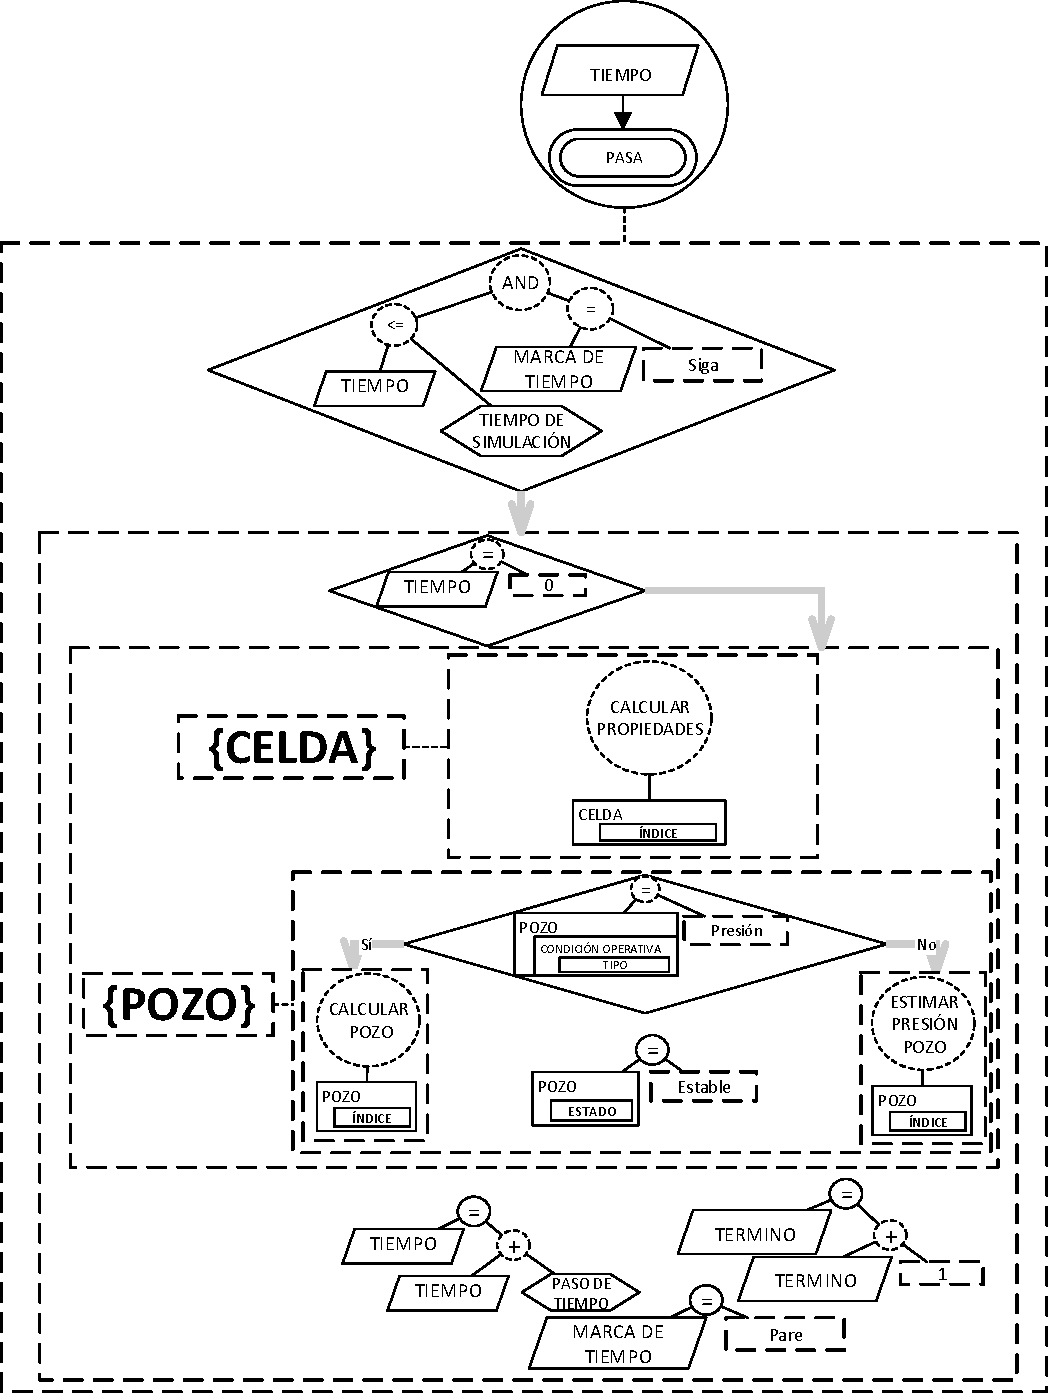
\includegraphics[width=0.7\linewidth]{Fig/TiempoPasa.pdf}%
	%\caption{Complete PS Representation for EOR Processes} \label{fig:PSComplete}
	\caption[Representación del paso del tiempo.]{Representación del paso del tiempo. Los autores.} \label{fig:TimePasses}
\end{figure}


\subsection{Presión del Fluido Varía}\label{sec:PS_FluidVaries}
En el evento ``Presión del Fluido varía'' se procesa el núcleo de la simulación. En éste se llevan a cabo las iteraciones del método de Newton-Raphson para converger al próximo paso de tiempo. La especificación de este evento consta de cinco procesos principales: La actualización de propiedades al término actual, el recálculo de las mismas, el cálculo de los residuales en cada iteración, el cálculo de la matriz jacobiana, y la actualización de las incógnitas. La especificación del evento ``Presión del Fluido varía'' se presenta en la figura \ref{fig:FluidPressureVaries}.\\

\begin{figure}[h]
	\centering%
	\includegraphics[width=0.9\linewidth]{Fig/PresionVaria.pdf}%
	%\caption{Complete PS Representation for EOR Processes} \label{fig:PSComplete}
	\caption[Especificación del evento Presión del fluido varía.]{Especificación del evento Presión del fluido varía. Los autores.} \label{fig:FluidPressureVaries}
\end{figure}

\subsubsection{Actualización de arreglos de propiedades}\label{subsec:PS_DefVars}
En la actualización de propiedades al término actual, se hace un incremento de tamaño y asignación del estimado inicial para el método de Newton-Raphson para todas las celdas de la malla y en todos los fluidos para todas las propiedades dependientes del tiempo. Lo mismo se realiza para los pozos y cada uno de sus perforados. La actualización de propiedades se expone en la figura \ref{fig:UpdateProperties}. 

\begin{figure}[h]
	\centering%
	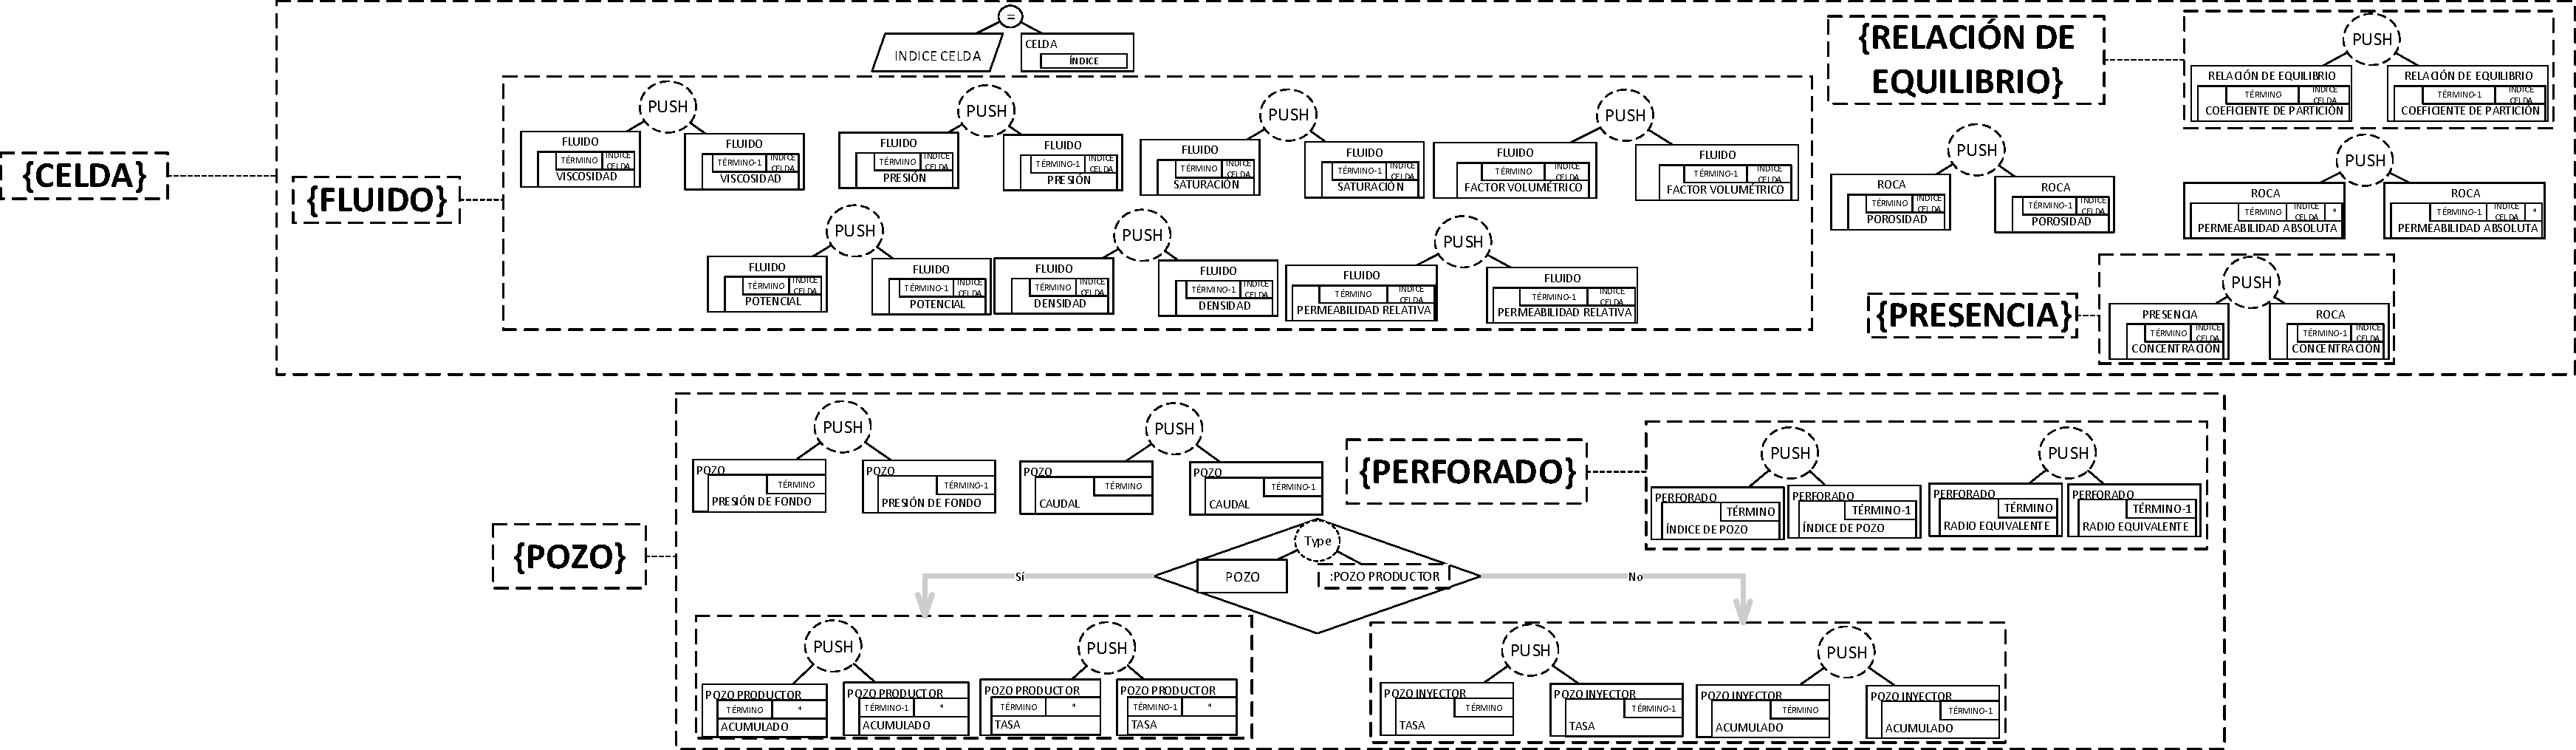
\includegraphics[width=\linewidth]{Fig/ActualizacionDeVariables.pdf}%
	%\caption{Complete PS Representation for EOR Processes} \label{fig:PSComplete}
	\caption[Actualización de propiedades al término actual.]{Actualización de propiedades al término actual. Los autores.} \label{fig:UpdateProperties}
\end{figure}


\subsubsection{Recálculo de propiedades de los fluidos}\label{subsec:PS_TimeK}
Posteriormente en la figura \ref{fig:TimeK} se muestra el recálculo de las propiedades de los fluidos para cada celda. Como el sistema que se resuelve tiene por incógnitas la presión del fluido principal y la saturación de los demás fluidos, es necesario calcular el resto de las propiedades de los fluidos como funciones de estas. \\%Time K

\begin{figure}[h]
	\centering%
	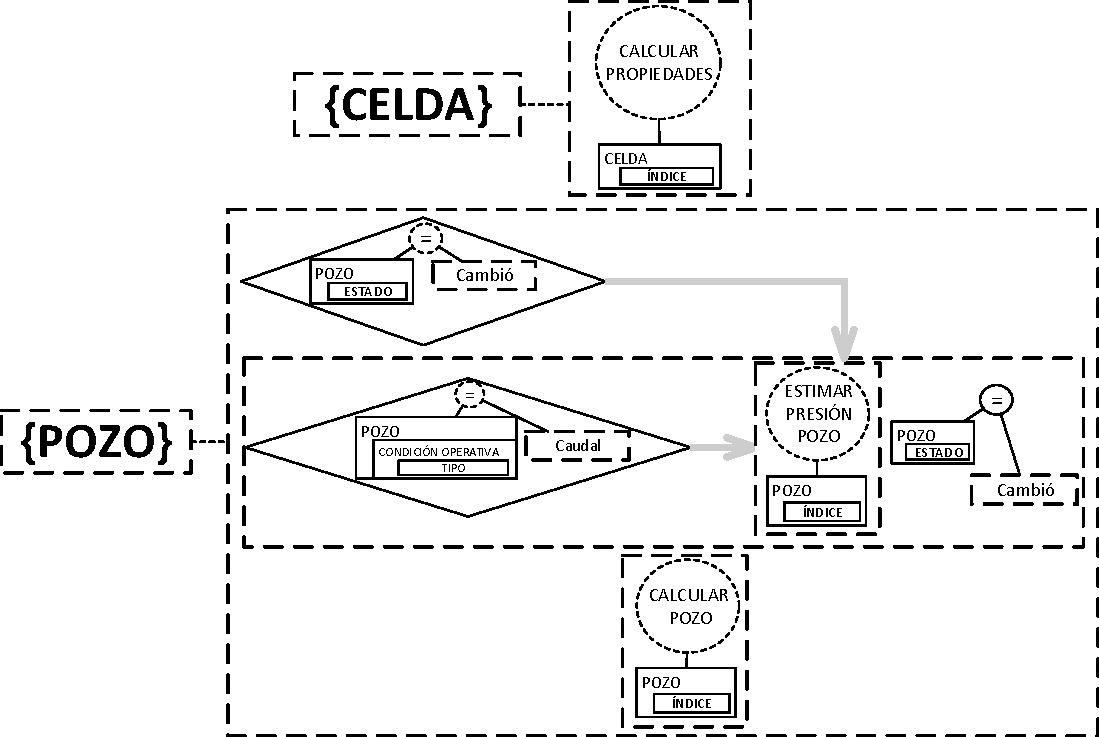
\includegraphics[width=\linewidth]{Fig/TiempoK.pdf}%
	%\caption{Complete PS Representation for EOR Processes} \label{fig:PSComplete}
	\caption[Recálculo de Propiedades al término actual para la iteración.]{Recálculo de Propiedades al término actual para la iteración. Los autores.} \label{fig:TimeK}
\end{figure}

\subsubsection{Cálculo de Residuales}\label{subsec:Residual}
Luego \ref{fig:Residual} \\ % Residual

\begin{figure}[h]
	\centering%
	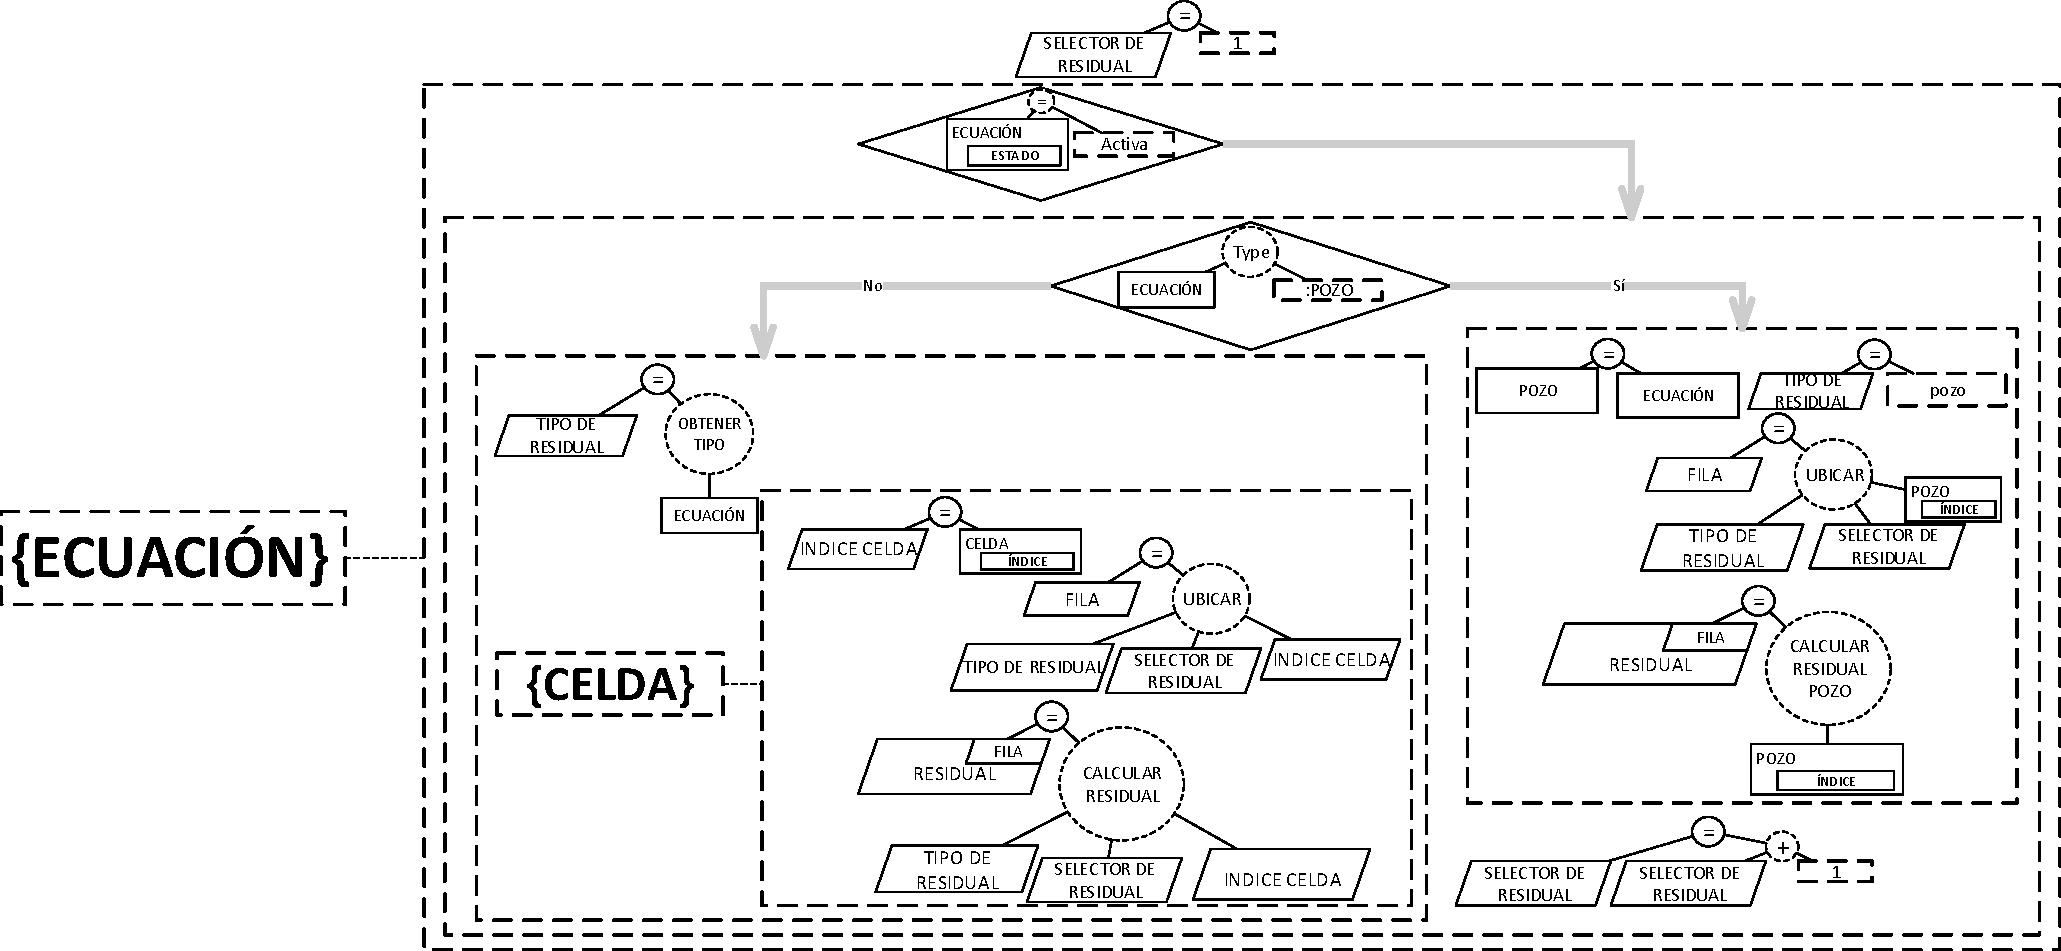
\includegraphics[width=\linewidth]{Fig/Residual.pdf}%
	%\caption{Complete PS Representation for EOR Processes} \label{fig:PSComplete}
	\caption[Cálculo de residual para la iteración.]{Cálculo de residual para la iteración. Los autores.} \label{fig:Residual}
\end{figure}

\subsubsection{Cálculo de la Matriz del Jacobiano}\label{subsec:Jacobian}
Siguiendo \ref{fig:Jacobiano} \\ % Jacobiano

\begin{figure}[h]
	\centering%
	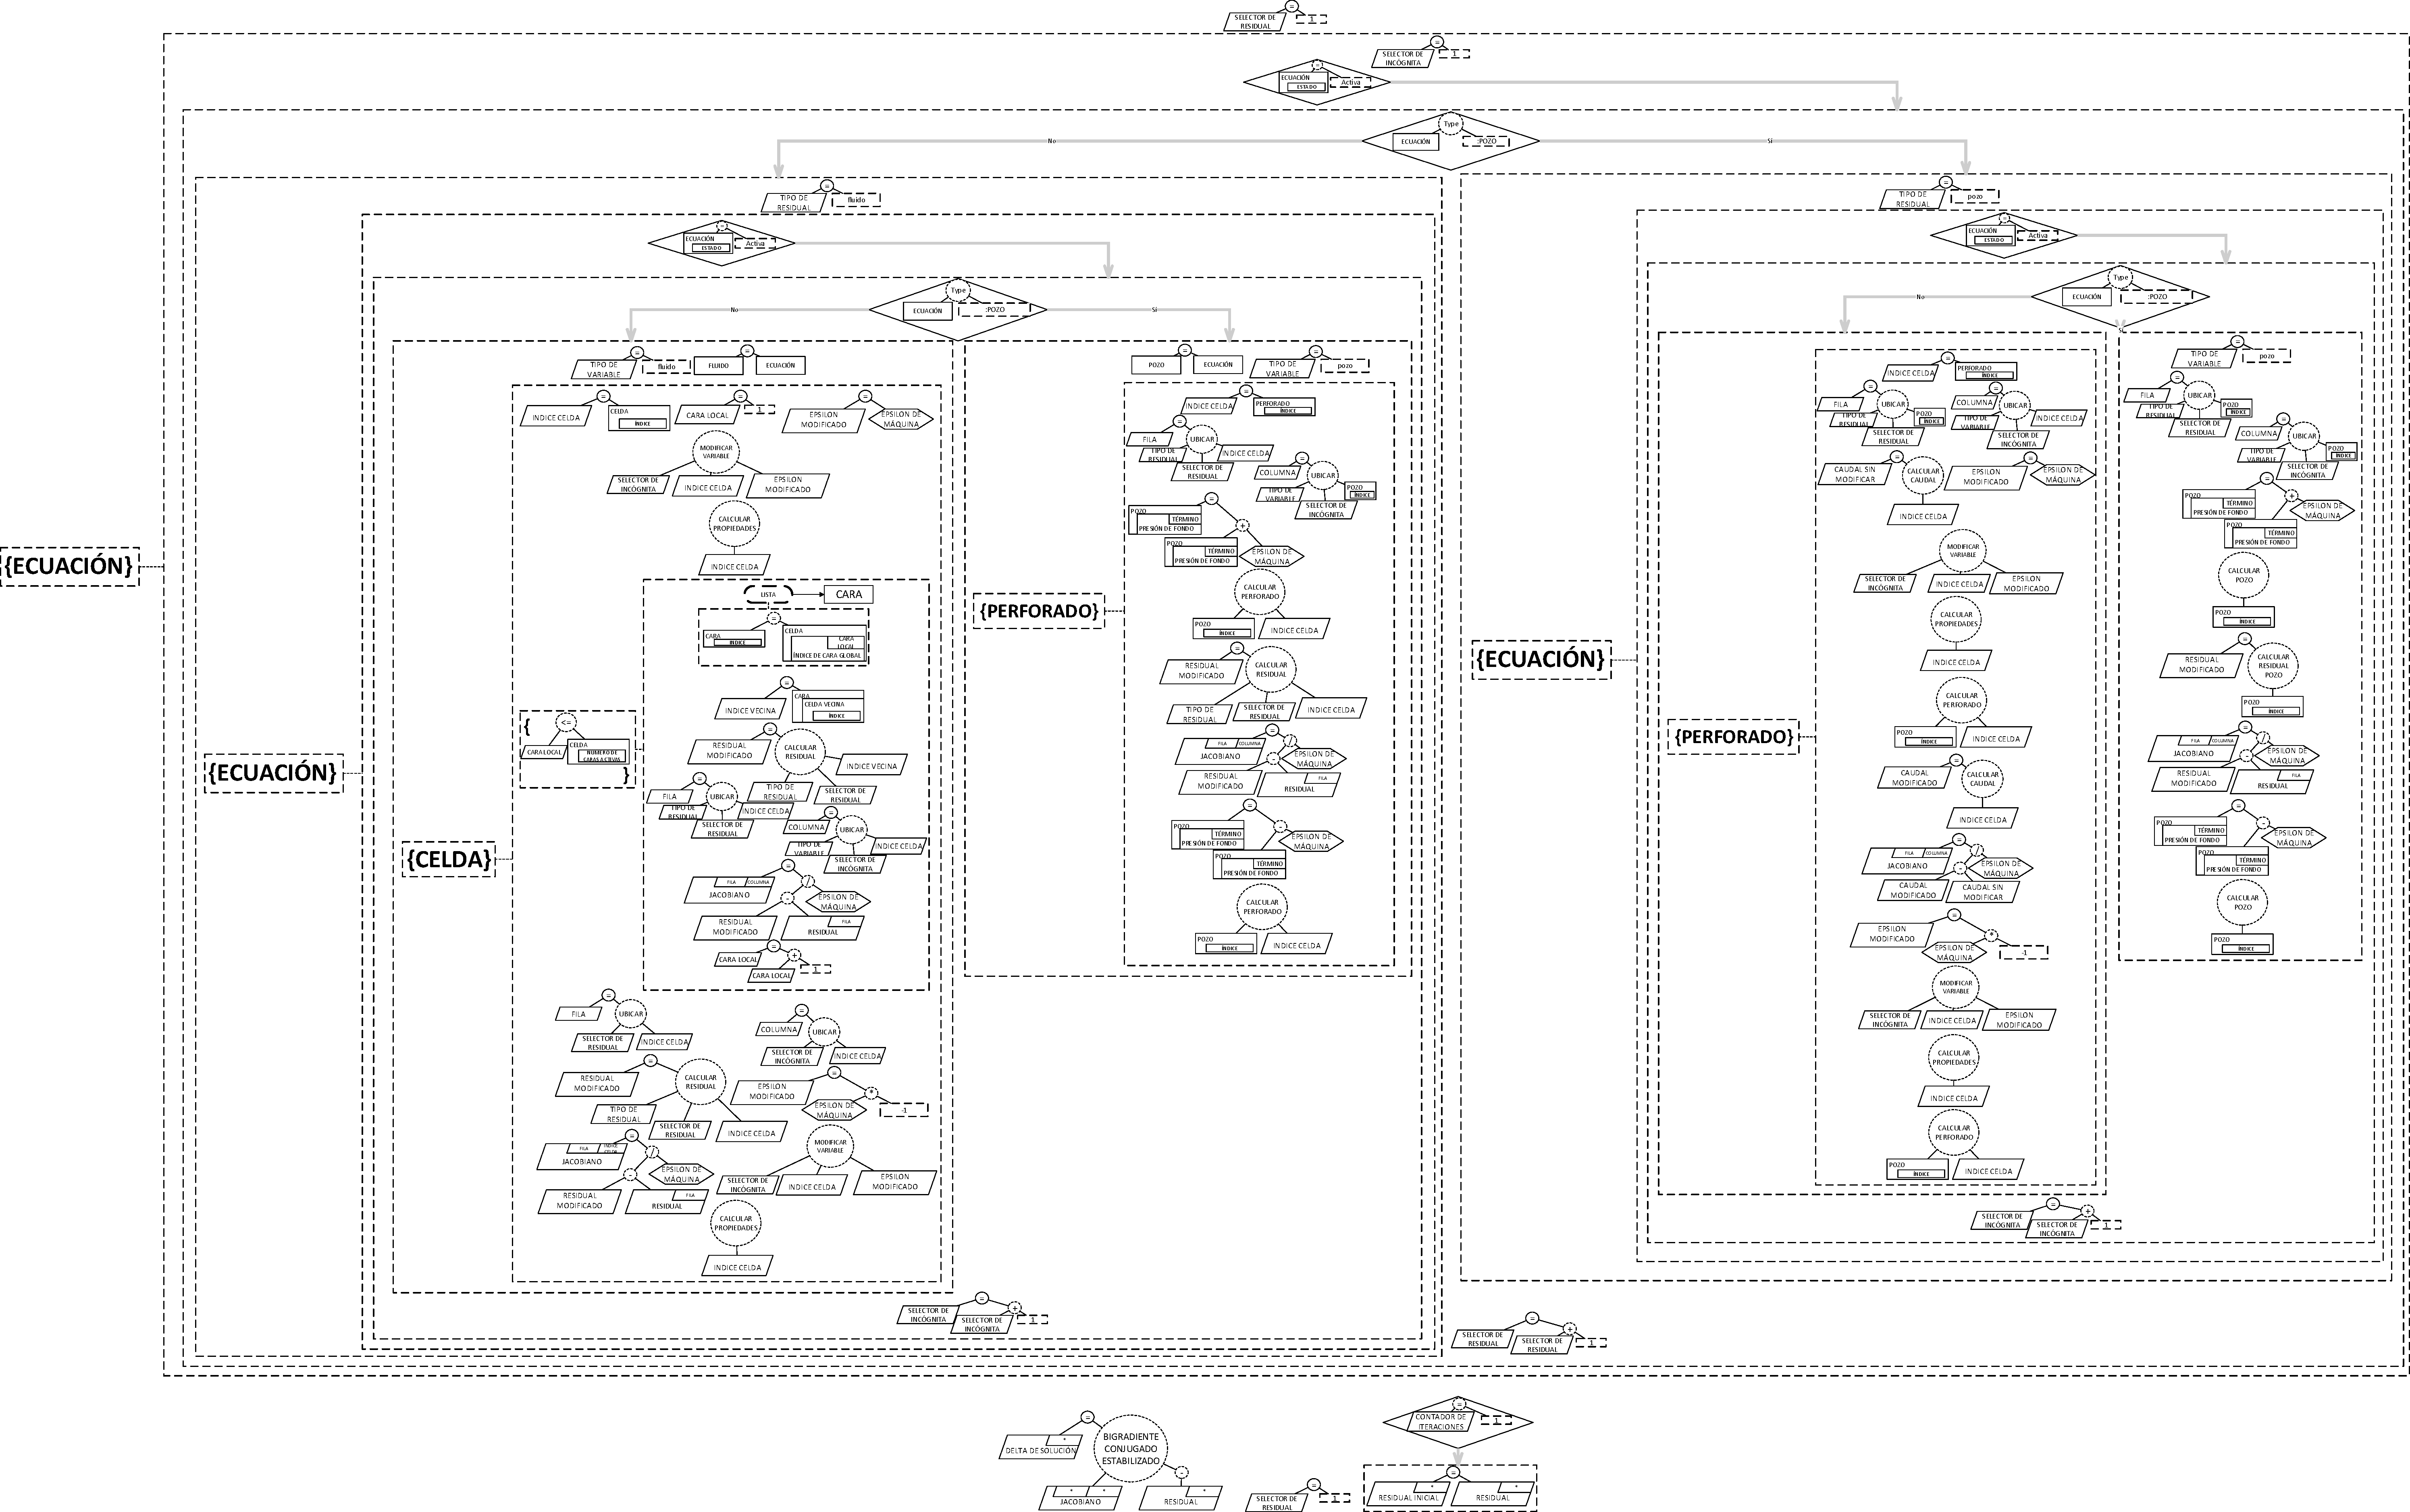
\includegraphics[width=\linewidth]{Fig/Jacobiano.pdf}%
	%\caption{Complete PS Representation for EOR Processes} \label{fig:PSComplete}
	\caption[Cálculo y armado de la matriz del jacobiano al término actual para la iteración.]{Cálculo y armado de la matriz del jacobiano al término actual para la iteración. Los autores.} \label{fig:Jacobiano}
\end{figure}

Por último \ref{fig:UpdateVariables} \\

\begin{figure}[h]
	\centering%
	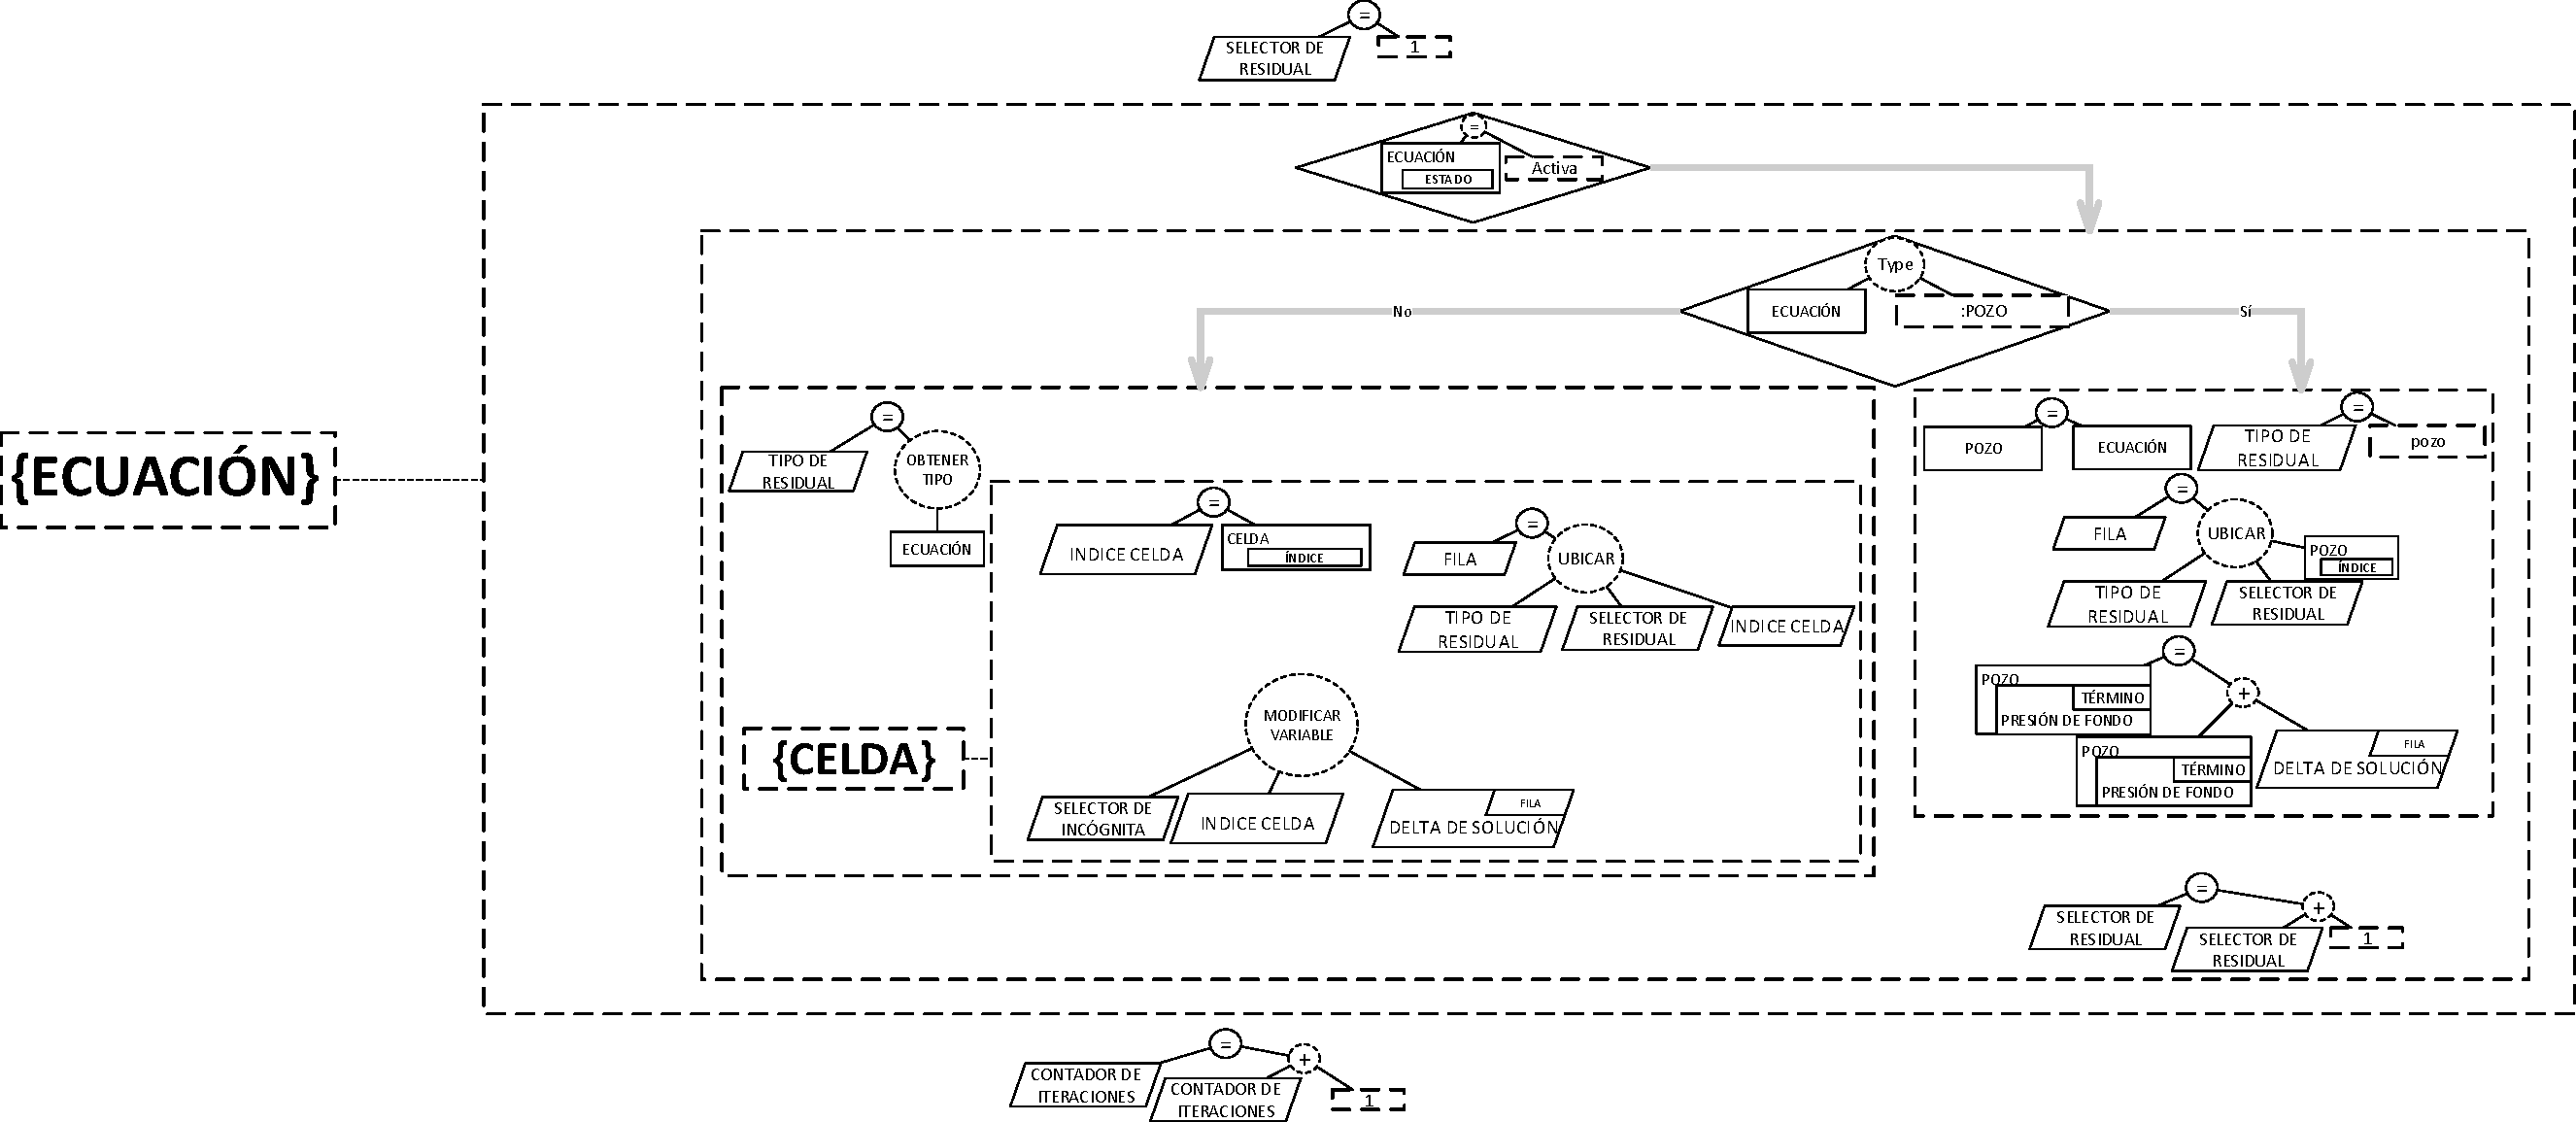
\includegraphics[width=\linewidth]{Fig/ActualizacionDeIncognitas.pdf}%
	%\caption{Complete PS Representation for EOR Processes} \label{fig:PSComplete}
	\caption[Recálculo de Propiedades al término actual para la iteración.]{Recálculo de Propiedades al término actual para la iteración. Los autores.} \label{fig:UpdateVariables}
\end{figure}
%includefigure{Graphical Representation of subroutine}

%includegraphic{Code Translation}

%Se deben incluir tantos cap\'{\i}tulos como se requieran; sin embargo, se recomienda que la tesis  o trabajo de investigaci\'{o}n tenga un m\'{\i}nimo 3 cap\'{\i}tulos y m\'{a}ximo de 6 cap\'{\i}tulos (incluyendo las conclusiones).\\